

\newpage
\begin{figure}[H]
\begin{tabular}{c}
  \fbox{  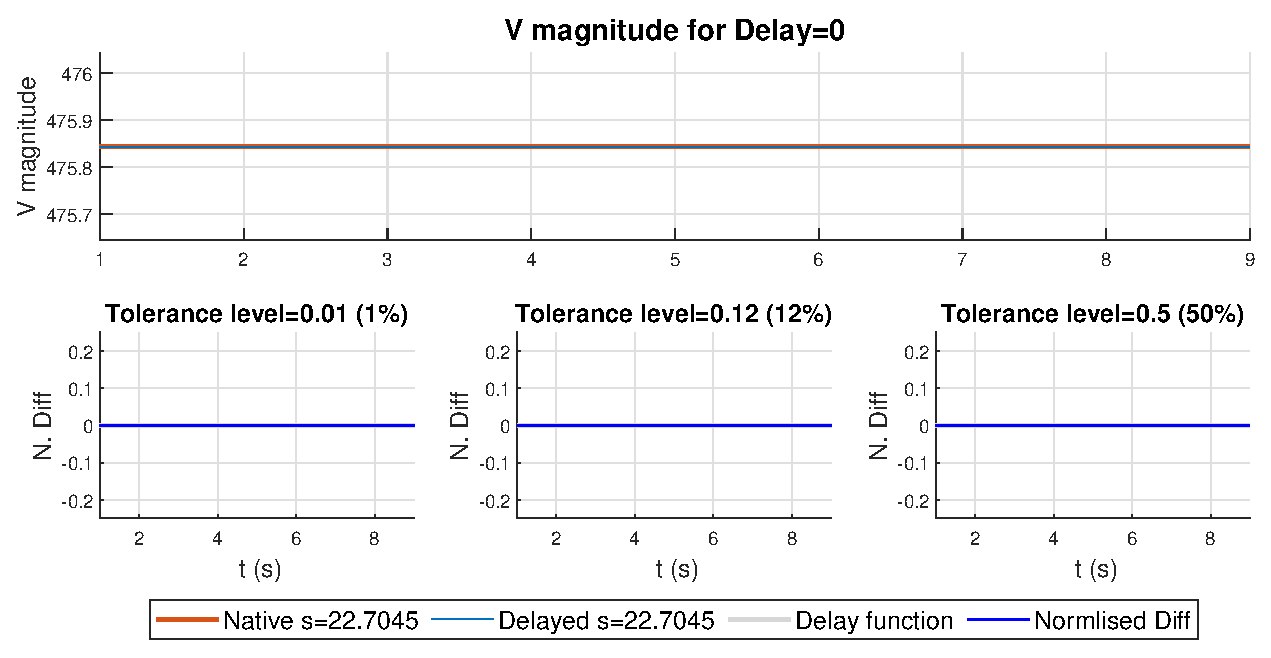
\includegraphics[width=0.95\textwidth]{PMUsim-figures/DelayOf_0/Zero_vMagnitude.eps}} \\ 
   
   \fbox{    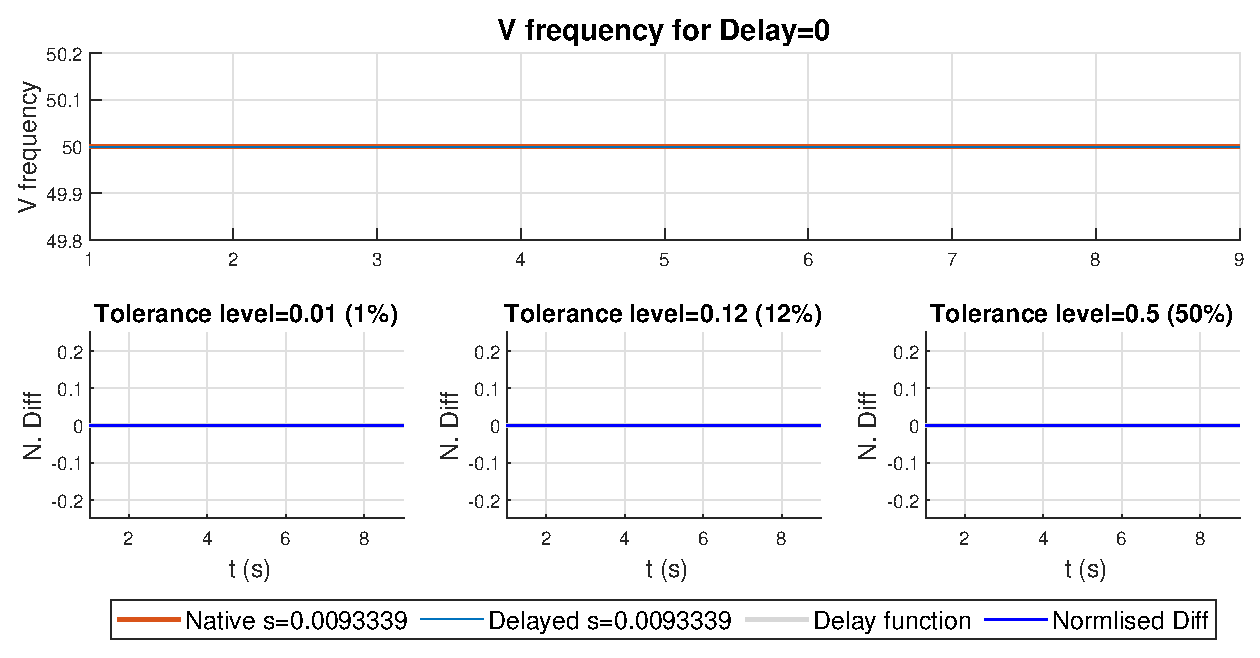
\includegraphics[width=0.95\textwidth]{PMUsim-figures/DelayOf_0/Zero_vFrequency.eps}} \\ 

   \fbox{     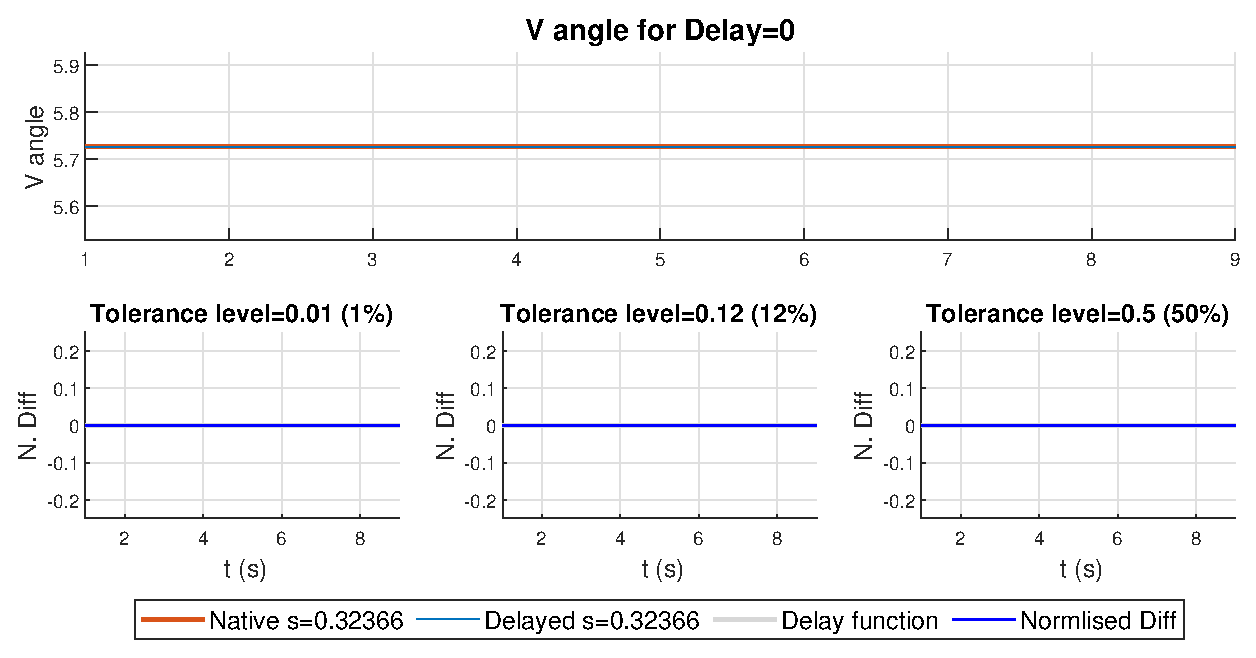
\includegraphics[width=0.95\textwidth]{PMUsim-figures/DelayOf_0/Zero_vAngle.eps}} 

  \end{tabular}
\caption{Results for Voltage Output for Delay equal to Zero }

     \tcbox[size=small, standard jigsaw, opacityback=0, boxrule=0pt,halign=justify]{
     Comments:}{
          \begin{itemize}
         \item      The delayed signal overlaps the original signal, producing a straight line colored in a different color from any of the colors in the associated legends.
         \item  The blue Normalised diff signal also overlaps the grey Zero delay function, with similar effects on the color of the line.
          \end{itemize} }

\label{fig:VoltageZeroDelay}
\end{figure}


\section{The Delay Level of Zero}
For model verification purposes, the output for the delay level of zero is included.

One could possibly dispute the relevance of including an attack producing a zero delay level, but the simulation is intended to serve two purposes, as previously explained in subsection \ref{subsec:ModelValidation}:

\begin{enumerate}
\item The design of the \textbf{DualPMU}  subsystem, as visualised in figure \ref{fig:DualPMU}, appears to include two instances of \acrlong{pmu}s of the same \acrshort{pmu} implementation, the SimScape Electric \acrshort{pmu} library module, as previously described in subsection \ref{subsec:ModelPMU}.  
\item The delay function, listed in \ref{tab:vDelay}, is presumably correct. Running a simulation with a constant delay level of Zero should produce the same result as for identical \acrfull{pmu}s, showing identical, and indistinguishable \acrshort{pmu} output, as displayed in the resulting figures.
\end{enumerate}

No matter how identical the \acrshort{pmu} implementations of the  \textbf{DualPMU}  subsystem appears to be: If the delay function erroneously introduces a delay, the resulting output of the simulation is unlikely to produce a correct result, 

The reverse argumentation also sounds reasonalbe:

No matter how perfect the delay function might be, if the simulation produces deviating results, erroneously indicating a, possibly random, delay, the \acrshort{pmu} implementations of the  \textbf{DualPMU}  subsystem  is unlikely to be correct. 

\subsubsection{Result for delay Zero:}

On the next, as well as the previous page, the results of running the simulation with a delay level of Zero is presented. Comments are located underneath the name of each figure.


\newpage
\begin{figure}[H]
\begin{tabular}{c}
    \fbox{ 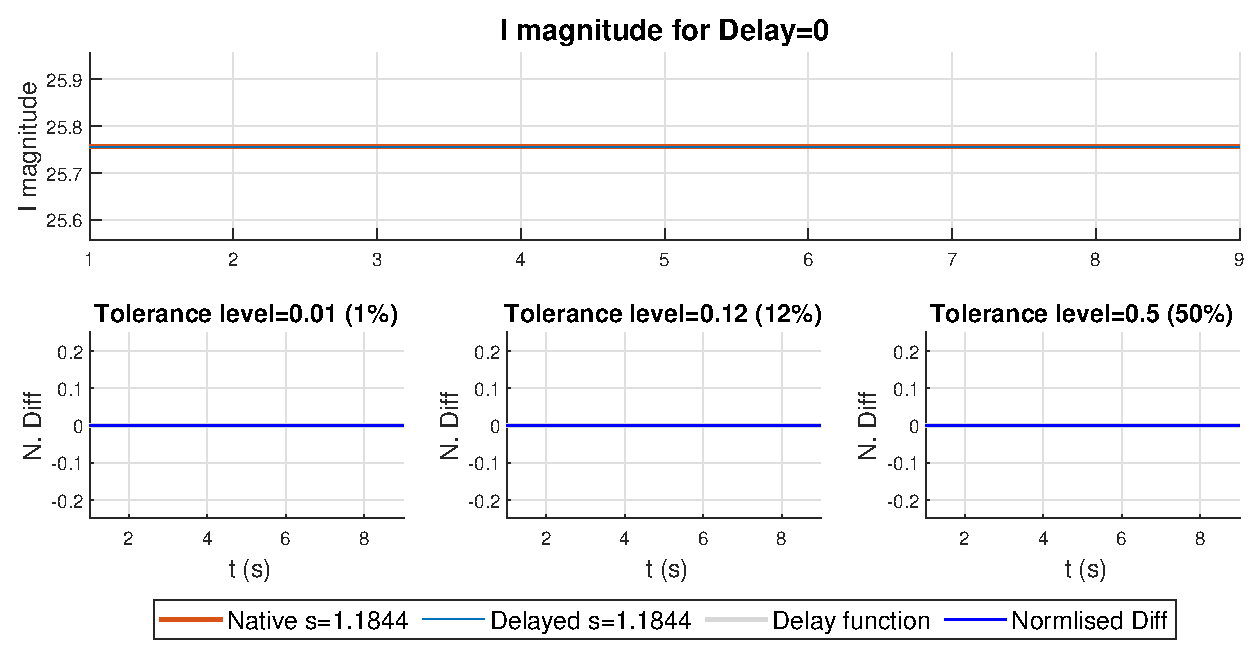
\includegraphics[width=0.95\textwidth]{PMUsim-figures/DelayOf_0/Zero_iMagnitude.eps}} \\
	
       \fbox{ 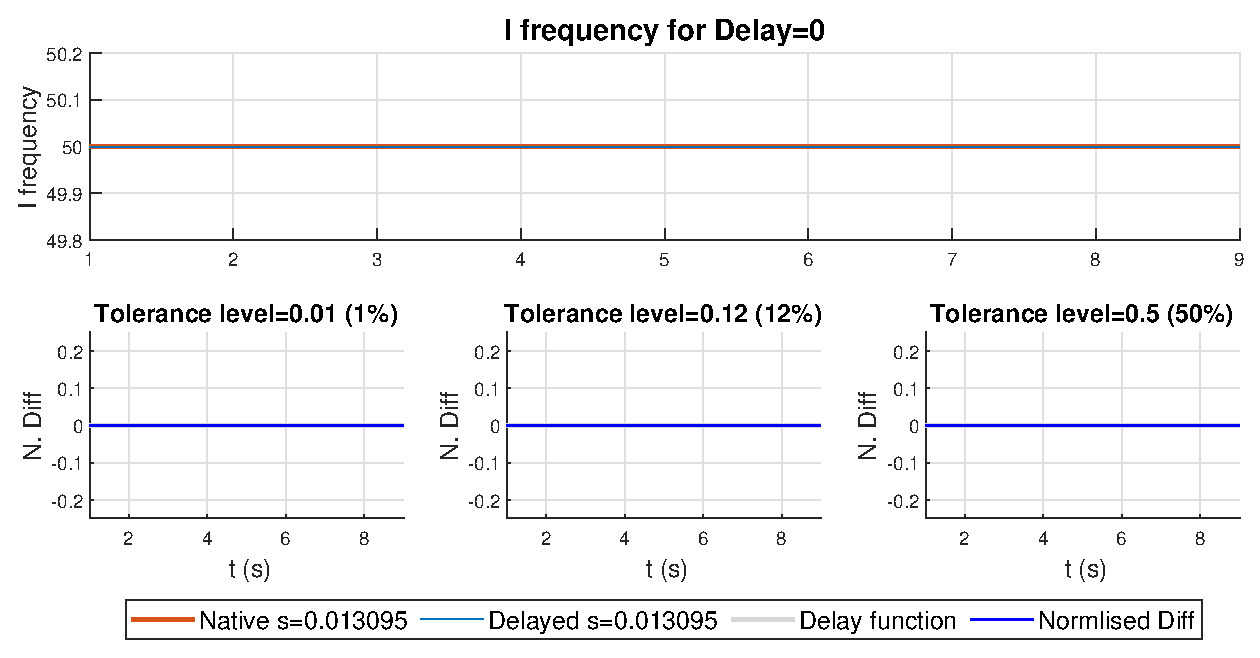
\includegraphics[width=0.95\textwidth]{PMUsim-figures/DelayOf_0/Zero_iFrequency.eps}}  \\
	   
   \fbox{  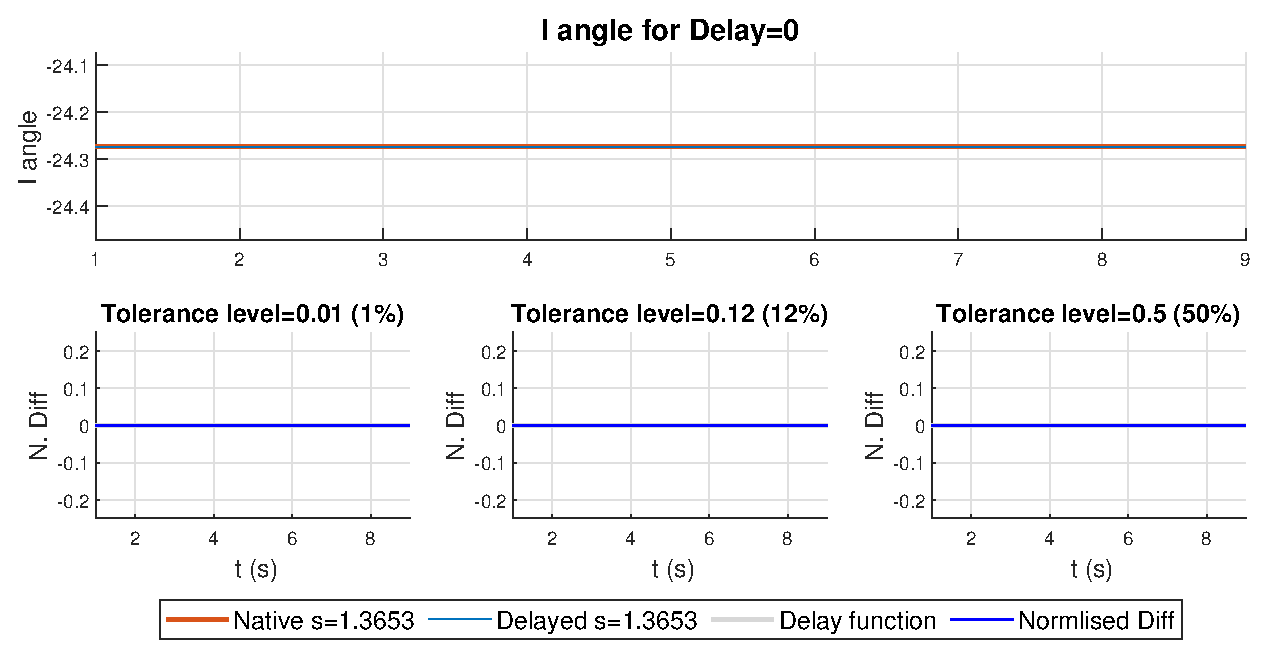
\includegraphics[width=0.95\textwidth]{PMUsim-figures/DelayOf_0/Zero_iAngle.eps}} \\ 


 %\caption{Zero Delay Frequency Output (for the Delay Level of Zero)}
  \end{tabular}
\caption{Results for Impedance Output for Delay equal to Zero }

     \tcbox[size=small, standard jigsaw, opacityback=0, boxrule=0pt,halign=justify]{
     Comments:}{
          \begin{itemize}
         \item      The delayed signal overlaps the original signal, producing a straight line colored in a different color from any of the colors in the associated legends.
         \item  The blue Normalised diff signal also overlaps the grey Zero delay function, with similar effects on the color of the line.
          \end{itemize} }

\label{fig:ImpedanceZeroDelay}
\end{figure}









\section{Instant Delay Simulations}
Instant delay simulations are characterised by the delay level instantly raises to the specified level, staying at the same constant level for the entire duration of the simulation, before instantly dropping to zero at the specified attack termination time.
The simulation focuses on:
\begin{itemize}
    \item Observing the situation prior to the attack for the purpose of comparing system state at attack termination with the pre-attack system state.
    \item observing the effect of a prolonged attack of constant level:
    \begin{itemize}
        \item What is the effect of a instant rise of the delay level for various delay levels?
        \item What is the effect of a instant drop of the delay level for various delay levels?
    \end{itemize}
\end{itemize}

On a suitable number of next pages, the figures showing the results of running the Instant Delay Simulations of levels One trough Six are available for inspection of the results. \\ Comments are located underneath the name of each figure.








\newpage
\begin{figure}[H]
\begin{tabular}{c}
  \fbox{  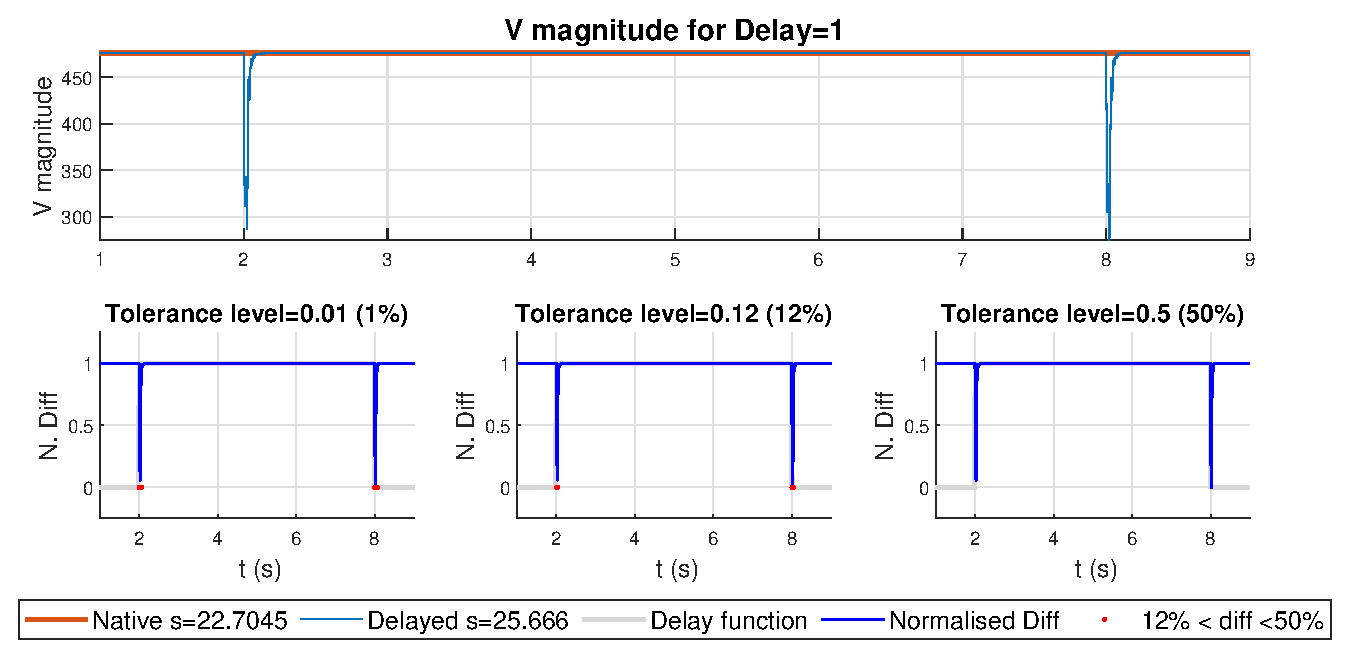
\includegraphics[width=0.95\textwidth]{PMUsim-figures/DelayOf_1/Instant_vMagnitude.eps}} \\ 
   \fbox{     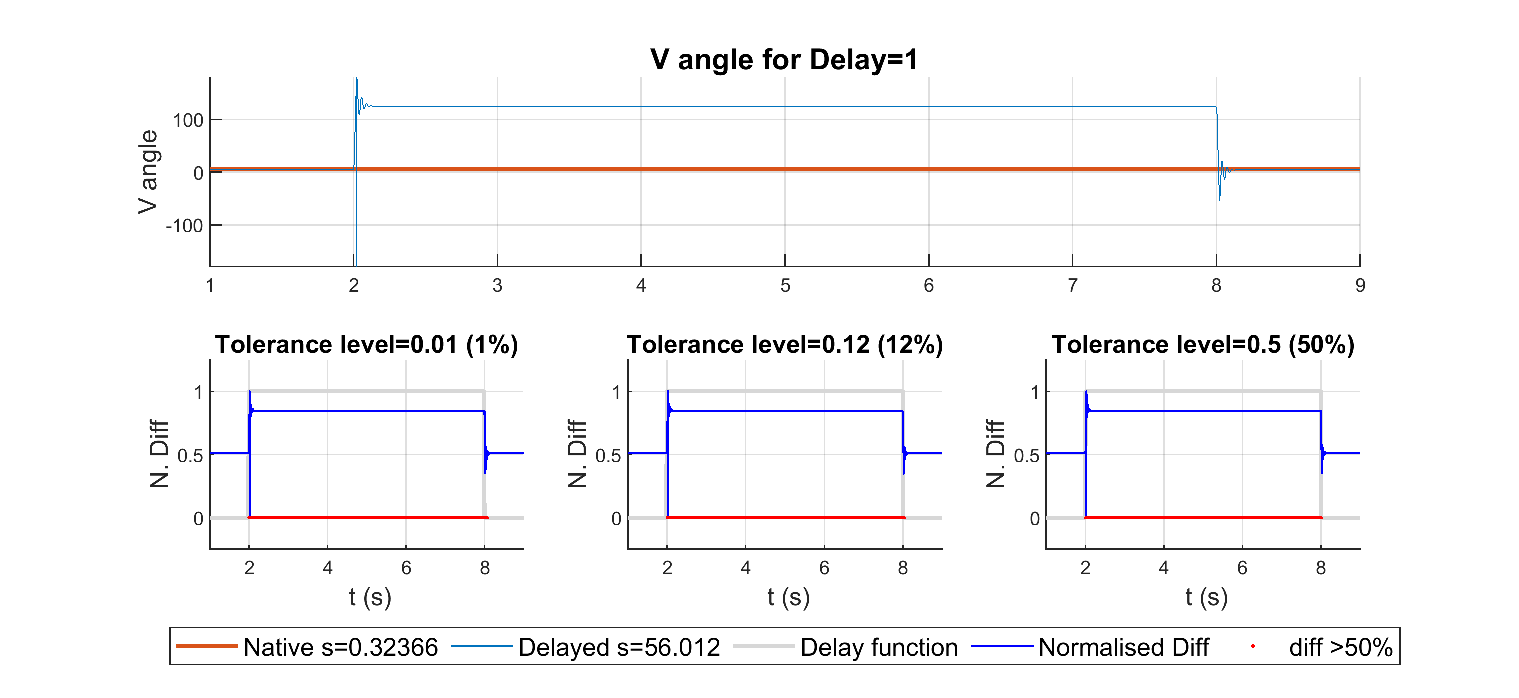
\includegraphics[width=0.95\textwidth]{PMUsim-figures/DelayOf_1/Instant_vAngle.eps}} \\   
   \fbox{    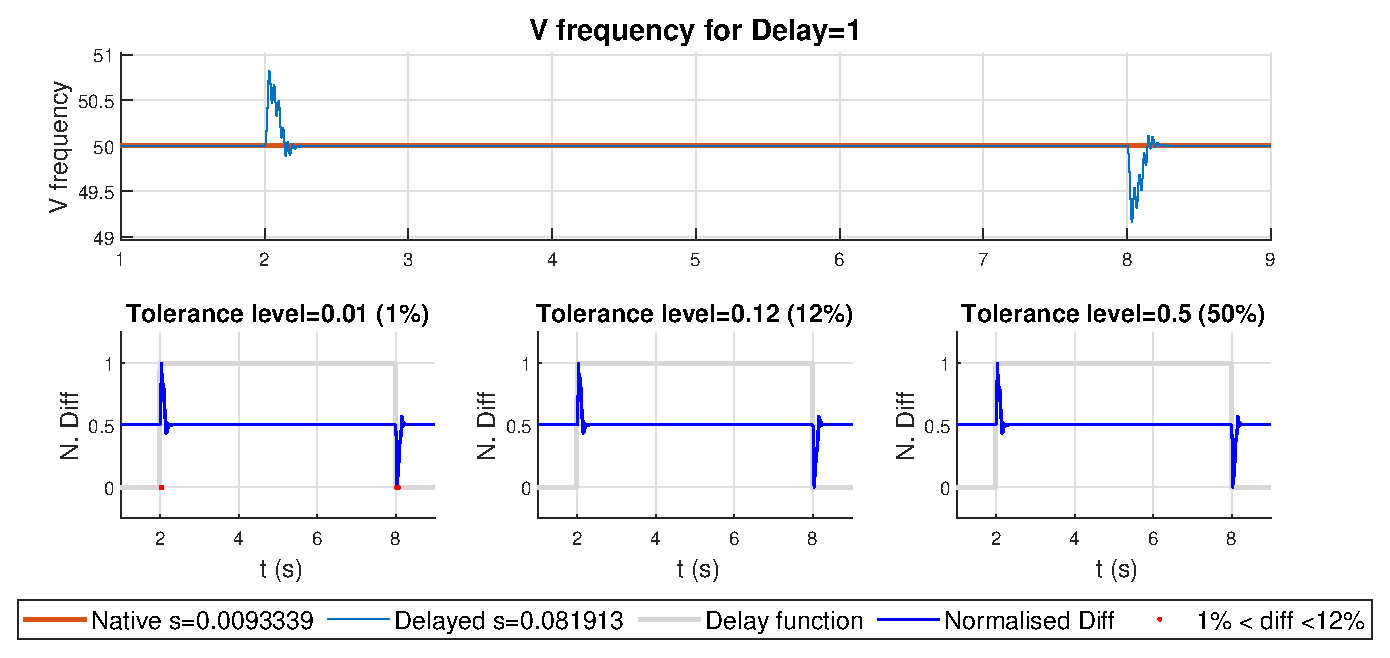
\includegraphics[width=0.95\textwidth]{PMUsim-figures/DelayOf_1/Instant_vFrequency.eps}}

 
  \end{tabular}
\caption{Results for Voltage Output for Instant Delay equal to One } 
\label{fig:VoltageInstantDelayOne}

     \tcbox[size=small, standard jigsaw, opacityback=0, boxrule=0pt,halign=justify]{
     Comments:}{
          \begin{itemize}
         \item      Apparently identical spikes are present for the magnitude graph, at initiation and termination of attack. 
         \item Similar, but mirrored, spikes are apparent for angle and frequency.
         \item  A constant shift of angle, possibly $120^0$, is apparent, whereas the other components, magnitude and frequency, shows no constant alteration of value.
          \end{itemize} }

\end{figure}

\newpage
\begin{figure}[H]
\begin{tabular}{c}
  \fbox{  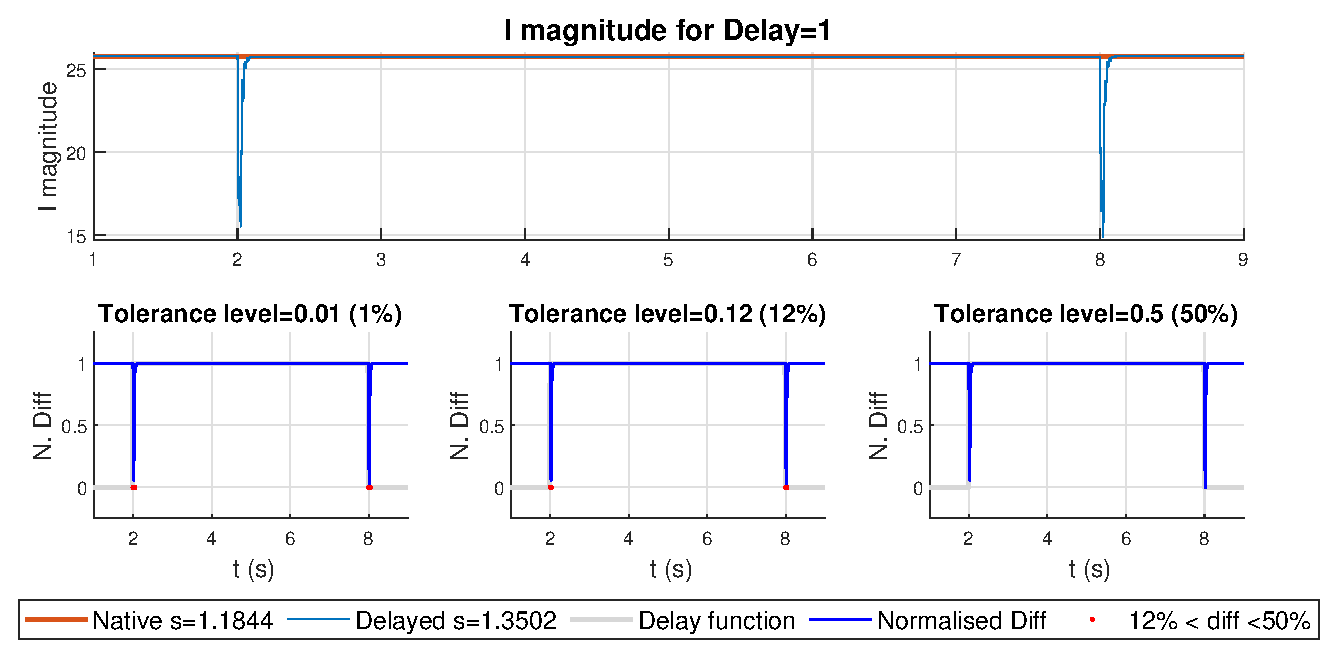
\includegraphics[width=0.95\textwidth]{PMUsim-figures/DelayOf_1/Instant_iMagnitude.eps}} \\ 
    \fbox{     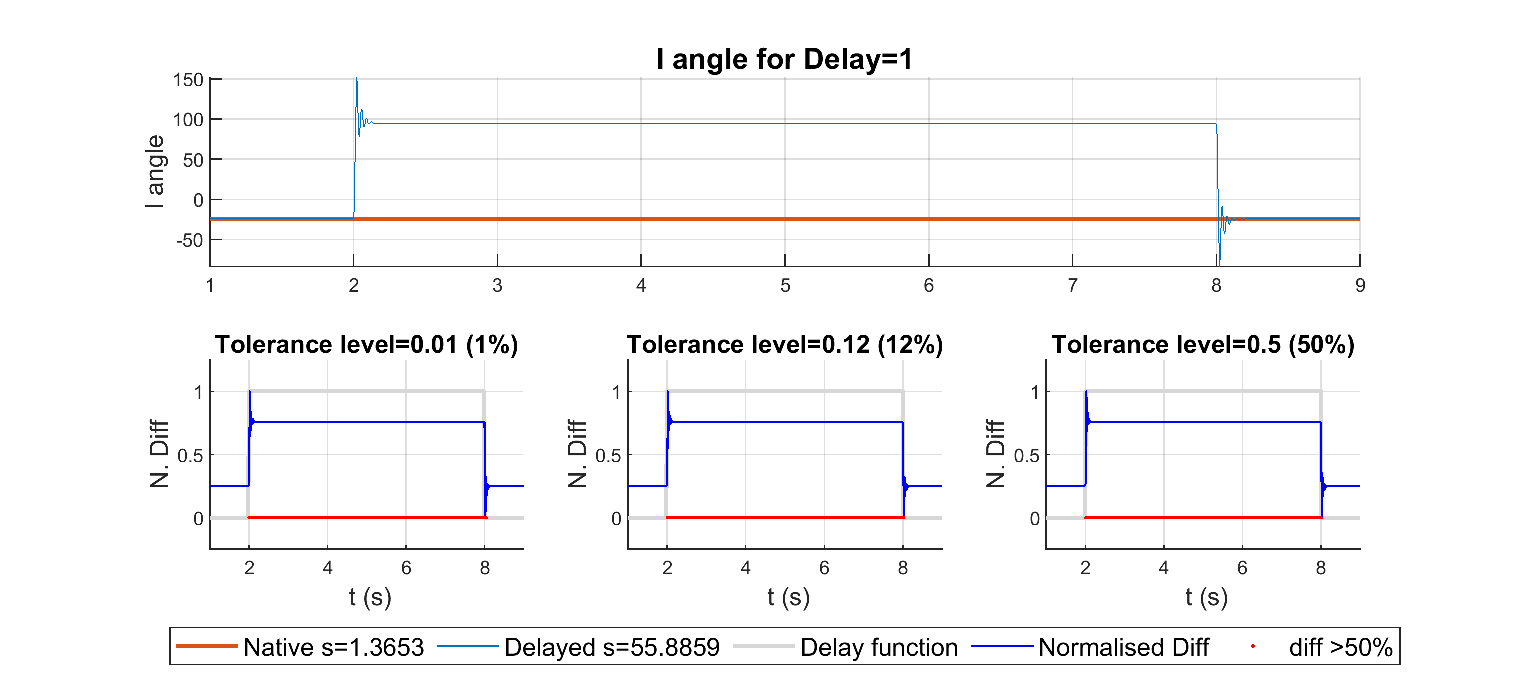
\includegraphics[width=0.95\textwidth]{PMUsim-figures/DelayOf_1/Instant_iAngle.eps}} \\   
   \fbox{    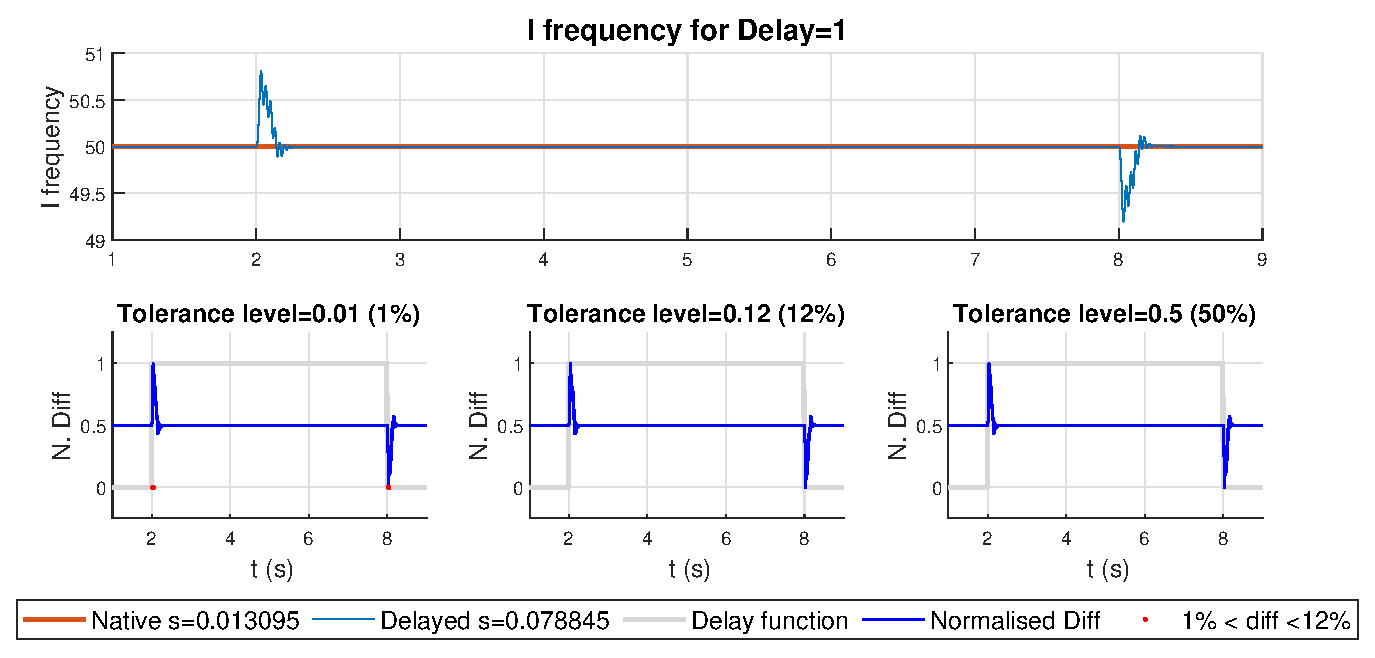
\includegraphics[width=0.95\textwidth]{PMUsim-figures/DelayOf_1/Instant_iFrequency.eps}}


  \end{tabular}
\caption{Results for Impedance Output for Instant Delay equal to One }
\label{fig:ImpedanceInstantDelayOne} 

     \tcbox[size=small, standard jigsaw, opacityback=0, boxrule=0pt,halign=justify]{
     Comments:}{
          \begin{itemize}
         \item      Apparently identical spikes are present for the magnitude graph, at initiation and termination of attack. 
         \item Similar, but mirrored, spikes are apparent for angle and frequency.
         \item  A constant shift of angle, possibly $120^0$, is apparent, whereas the other components, magnitude and frequency, shows no constant alteration of value.
          \end{itemize} }

\end{figure}



\newpage
\begin{figure}[H]
\begin{tabular}{c}
  \fbox{  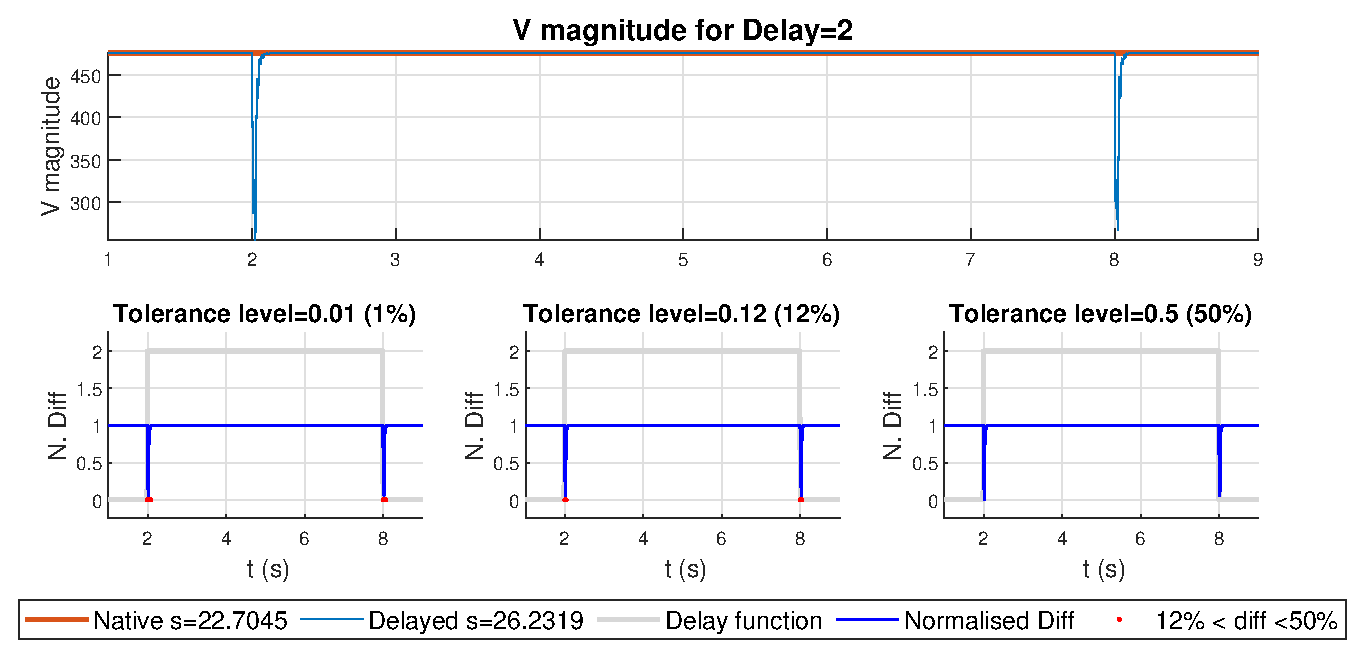
\includegraphics[width=0.95\textwidth]{PMUsim-figures/DelayOf_2/Instant_vMagnitude.eps}} \\ 
    \fbox{     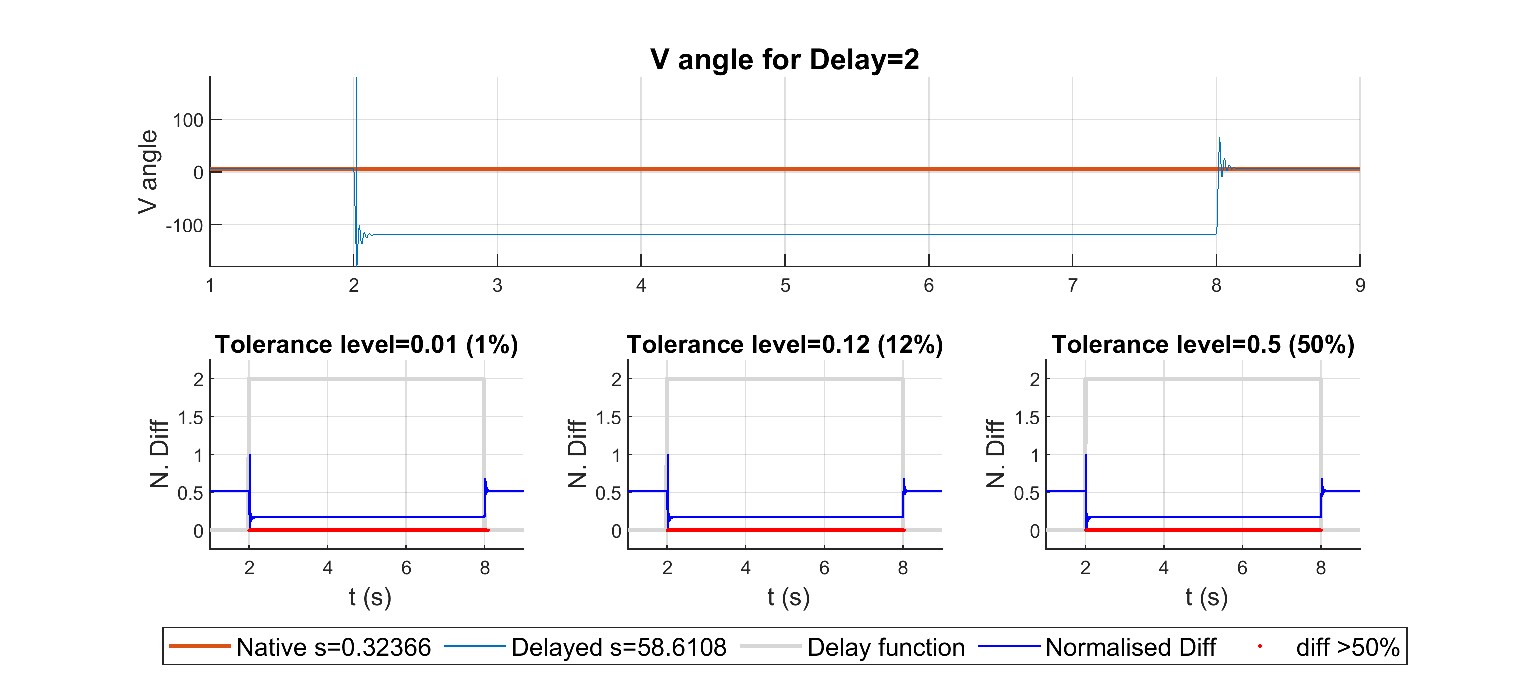
\includegraphics[width=0.95\textwidth]{PMUsim-figures/DelayOf_2/Instant_vAngle.eps}} \\  
   \fbox{    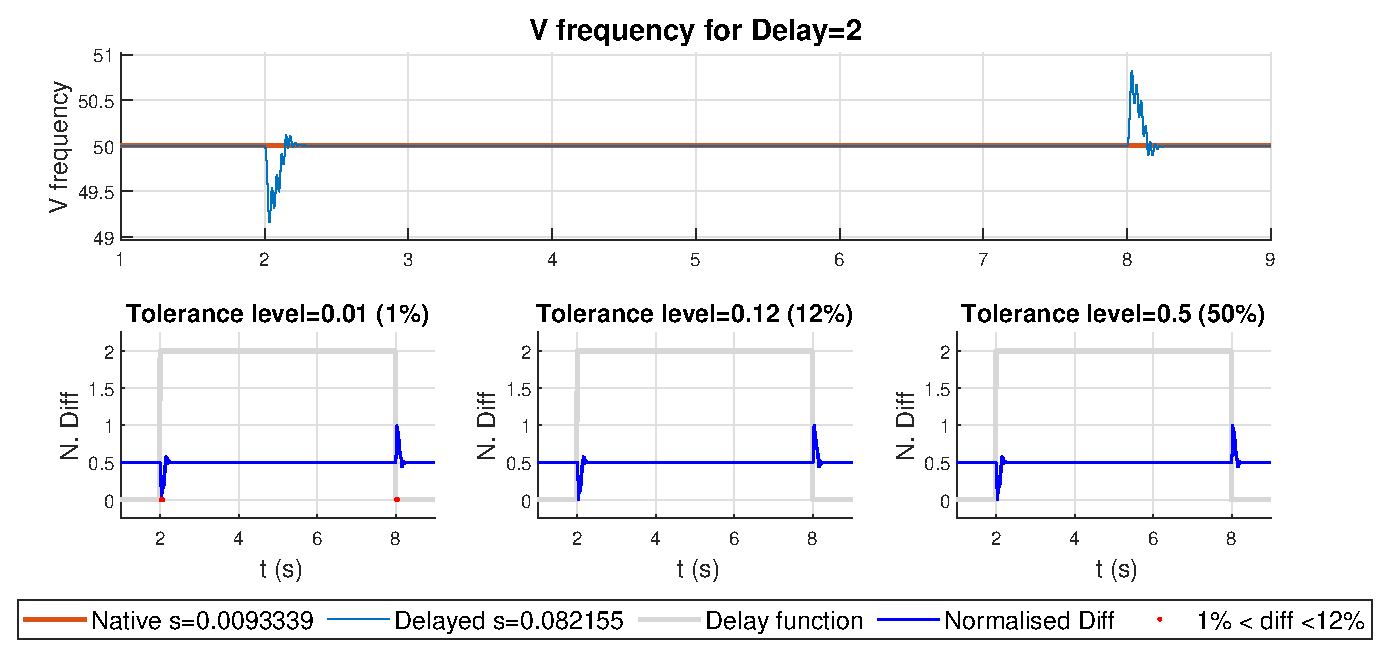
\includegraphics[width=0.95\textwidth]{PMUsim-figures/DelayOf_2/Instant_vFrequency.eps}}

 
  \end{tabular}
\caption{Results for Voltage Output for Instant Delay equal to Two }
\label{fig:VoltageInstantDelayTwo}

     \tcbox[size=small, standard jigsaw, opacityback=0, boxrule=0pt,halign=justify]{
     Comments:}{
          \begin{itemize}
         \item      Apparently identical spikes are present for the magnitude graph, at initiation and termination of attack. 
         \item Similar, but mirrored, spikes are apparent for the frequency, whereas the spikes for angle differs.
         \item  A constant shift of angle, possibly $-120^0$, is apparent, whereas the magnitude and frequency shows no constant alteration of value during the main period of the attack.
          \end{itemize} }
\end{figure}

\newpage
\begin{figure}[H]
\begin{tabular}{c}
  \fbox{  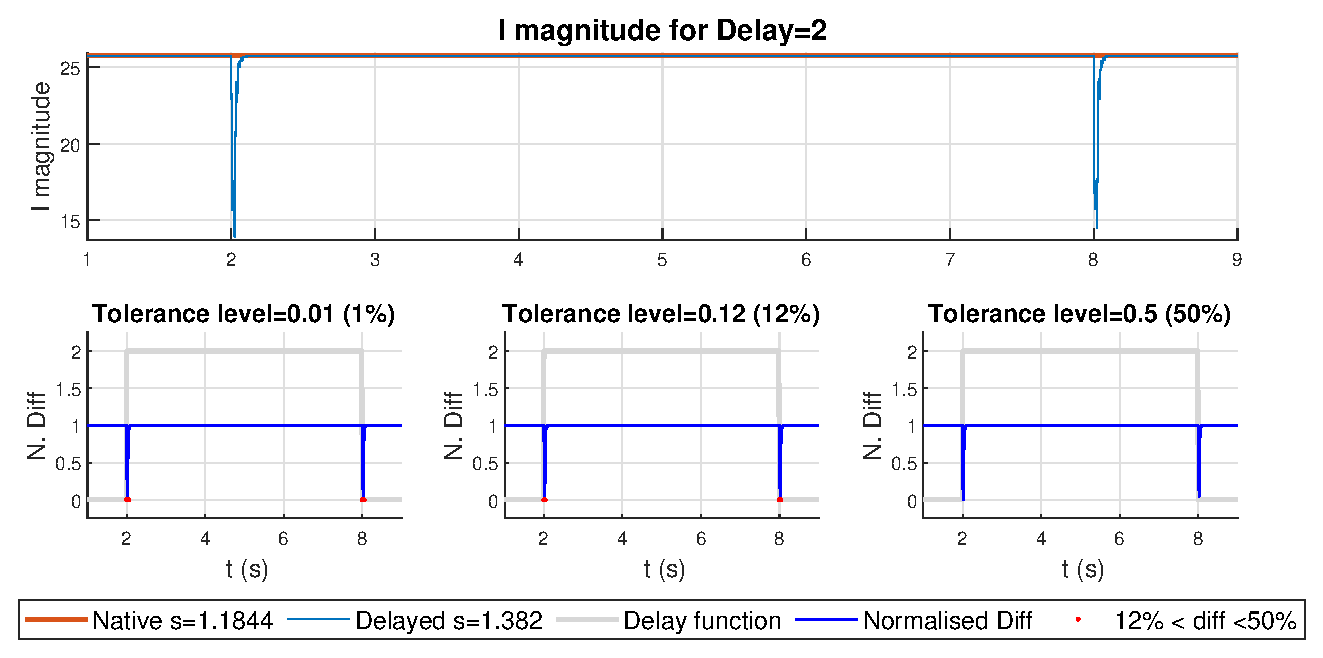
\includegraphics[width=0.95\textwidth]{PMUsim-figures/DelayOf_2/Instant_iMagnitude.eps}} \\ 
    \fbox{     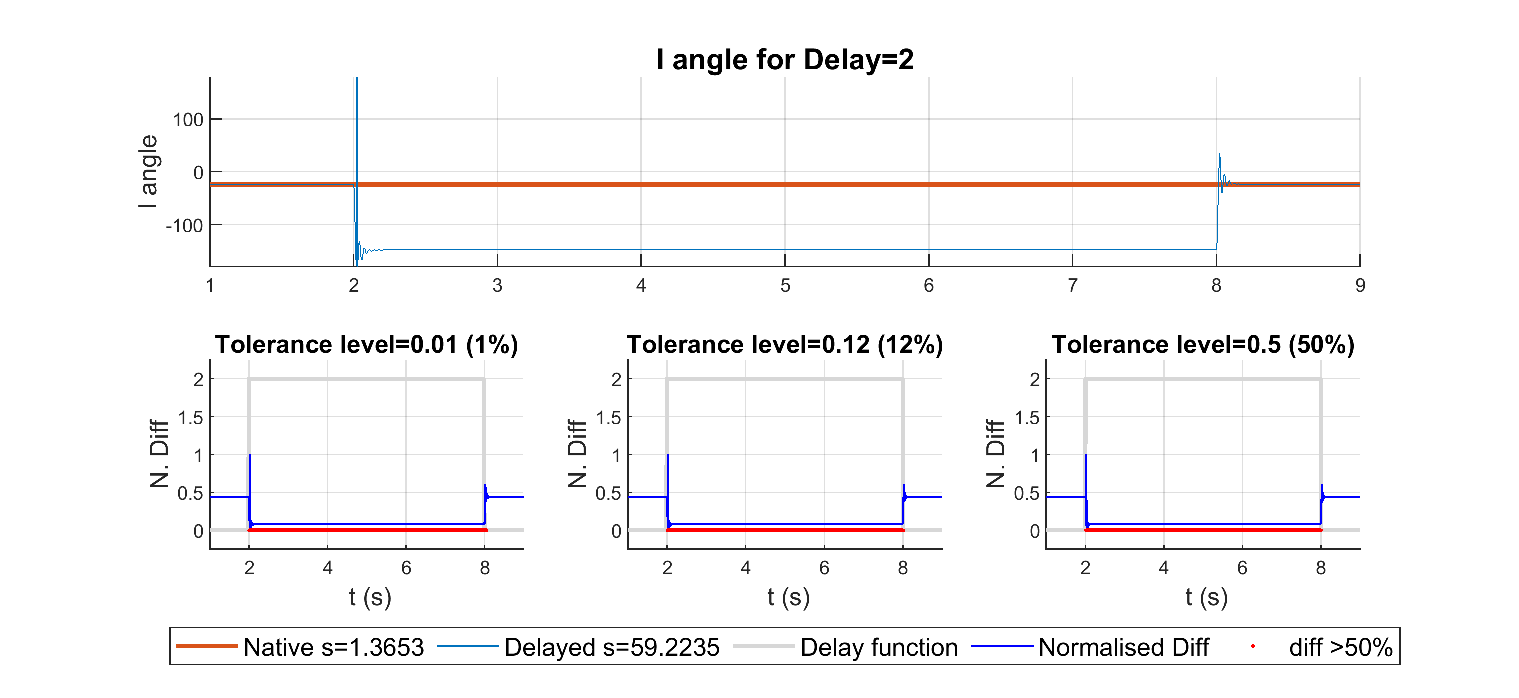
\includegraphics[width=0.95\textwidth]{PMUsim-figures/DelayOf_2/Instant_iAngle.eps}} \\   
   \fbox{    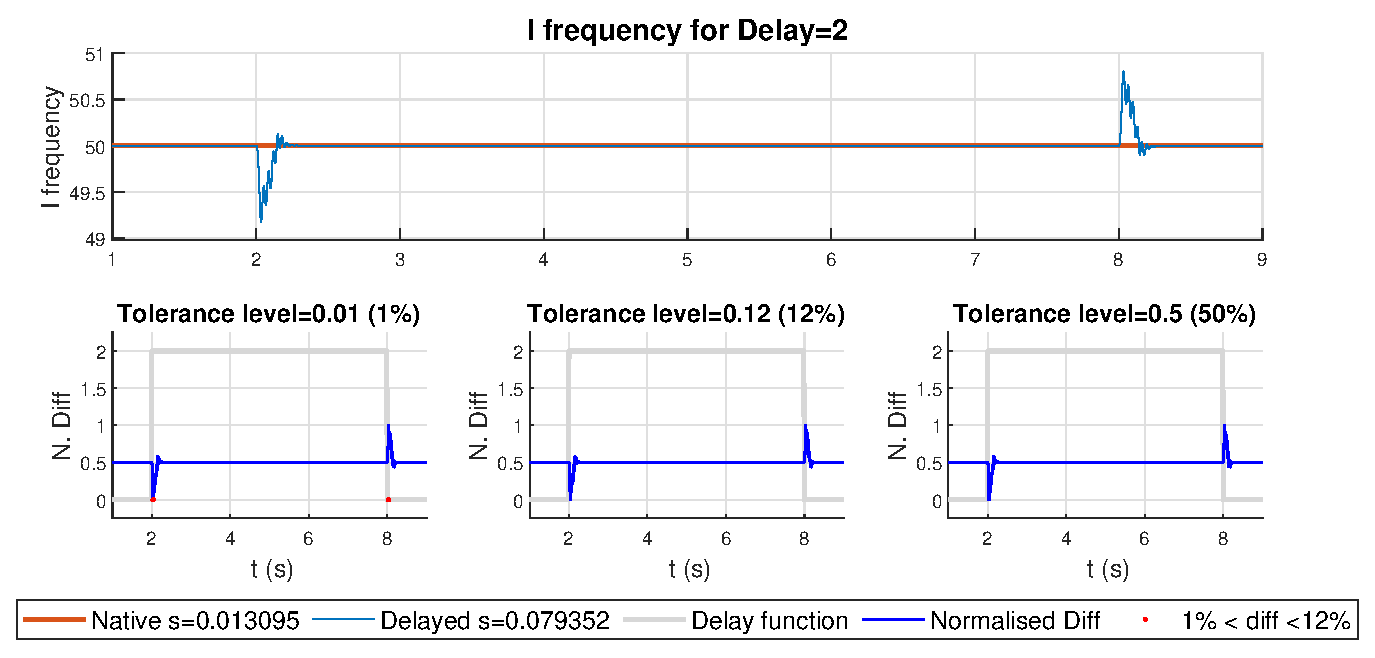
\includegraphics[width=0.95\textwidth]{PMUsim-figures/DelayOf_2/Instant_iFrequency.eps}}


  \end{tabular}
\caption{Results for Impedance Output for Instant Delay equal to Two }
\label{fig:ImpedanceInstantDelayTwo}

     \tcbox[size=small, standard jigsaw, opacityback=0, boxrule=0pt,halign=justify]{
     Comments:}{
          \begin{itemize}
         \item      Apparently identical spikes are present for the magnitude graph, at initiation and termination of attack. 
         \item Similar, but mirrored, spikes are apparent for the frequency, whereas the spikes for angle differs.
         \item  A constant shift of angle, possibly $-120^0$, is apparent, whereas the magnitude and frequency shows no constant alteration of value during the main period of the attack.
          \end{itemize} }

\end{figure}





\newpage
\begin{figure}[H]
\begin{tabular}{c}
  \fbox{  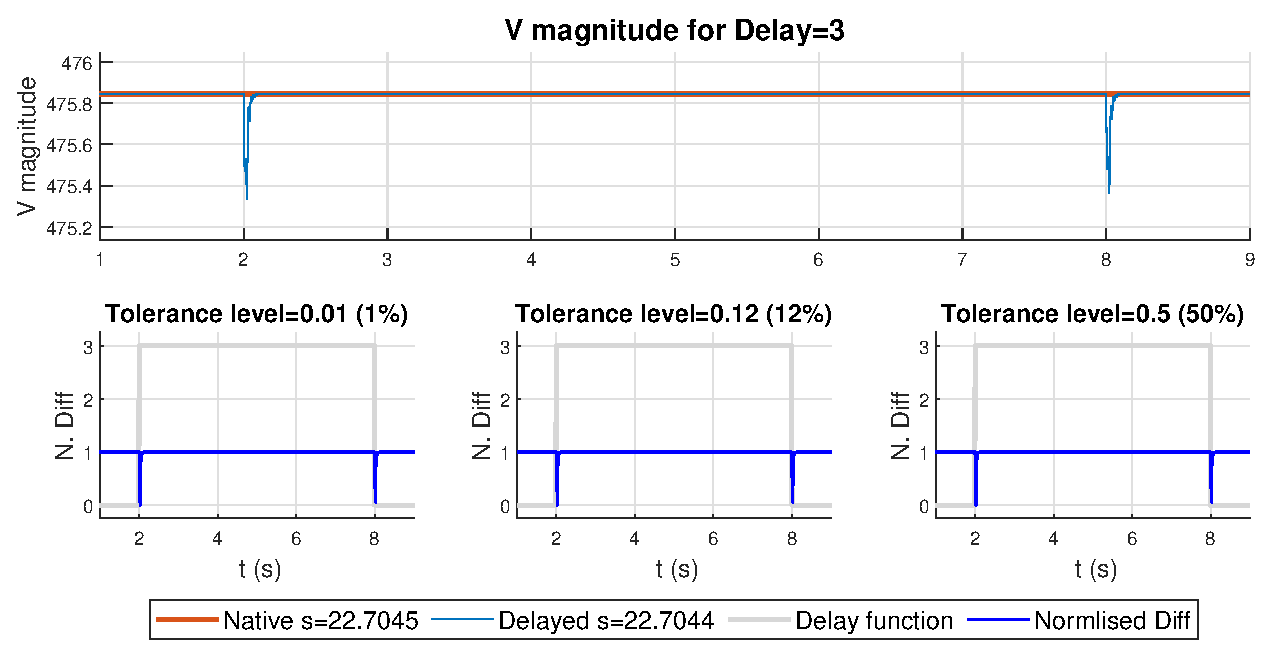
\includegraphics[width=0.95\textwidth]{PMUsim-figures/DelayOf_3/Instant_vMagnitude.eps}} \\ 
   \fbox{     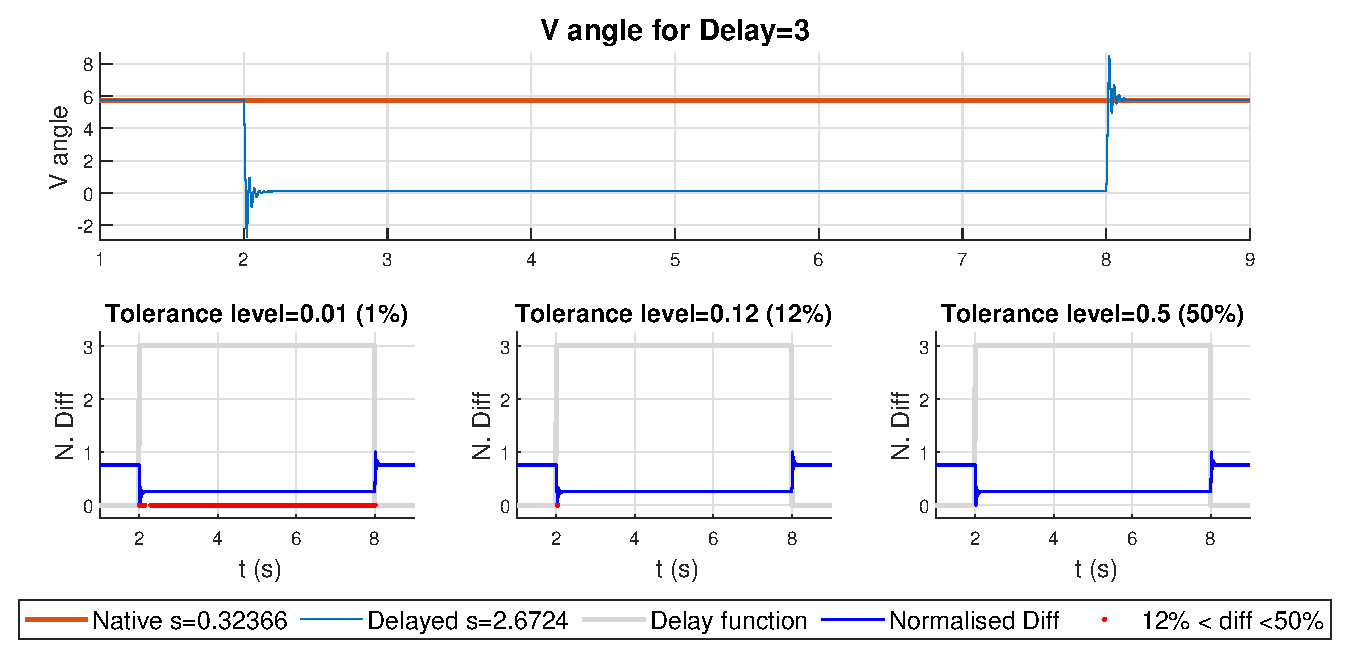
\includegraphics[width=0.95\textwidth]{PMUsim-figures/DelayOf_3/Instant_vAngle.eps}} \\    
   \fbox{    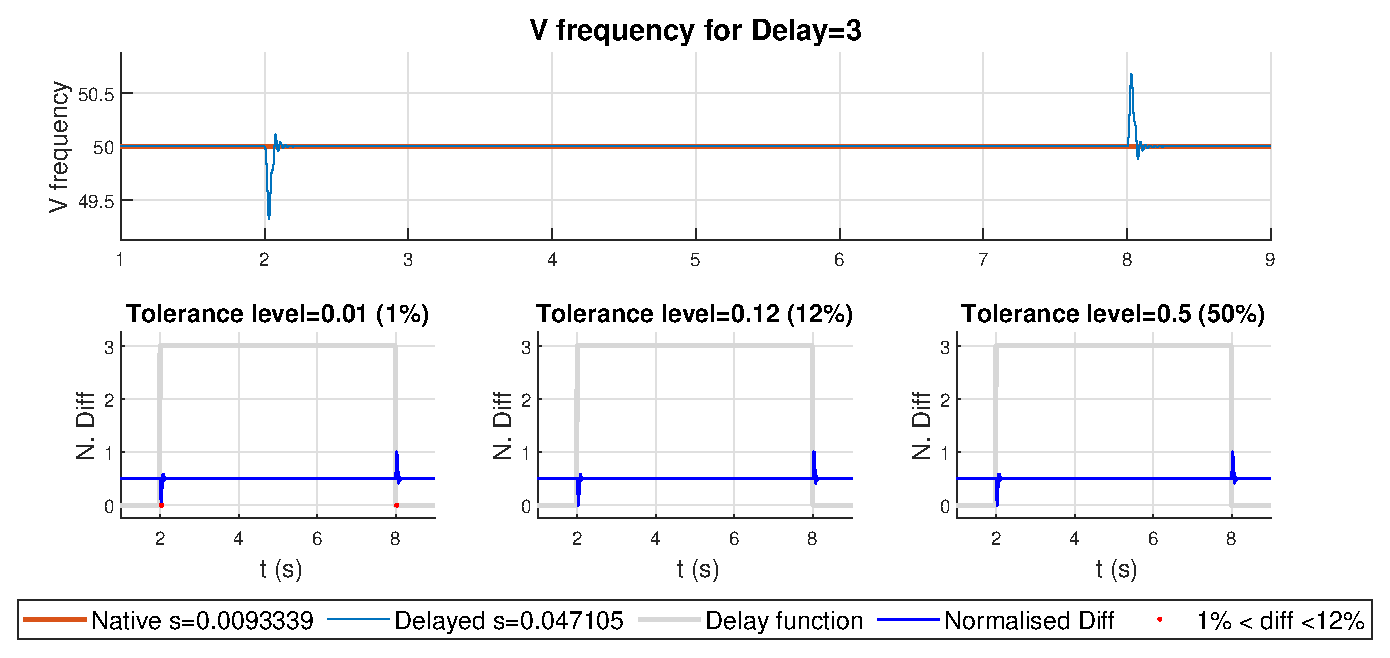
\includegraphics[width=0.95\textwidth]{PMUsim-figures/DelayOf_3/Instant_vFrequency.eps}}


  \end{tabular}
\caption{Results for Voltage Output for Instant Delay equal to Three }
\label{fig:VoltageInstantDelayThree}

     \tcbox[size=small, standard jigsaw, opacityback=0, boxrule=0pt,halign=justify]{
     Comments:}{
          \begin{itemize}
         \item      Apparently identical spikes are present for the magnitude graph, at initiation and termination of attack. 
         \item Similar, but mirrored, spikes are apparent for the frequency, whereas the spikes for angle differs.
         \item  A small constant shift of angle, possibly $-10^0$, is apparent, whereas the magnitude and frequency shows no constant alteration of value during the main period of the attack.
          \end{itemize} }
\end{figure}

\newpage
\begin{figure}[H]
\begin{tabular}{c}
  \fbox{  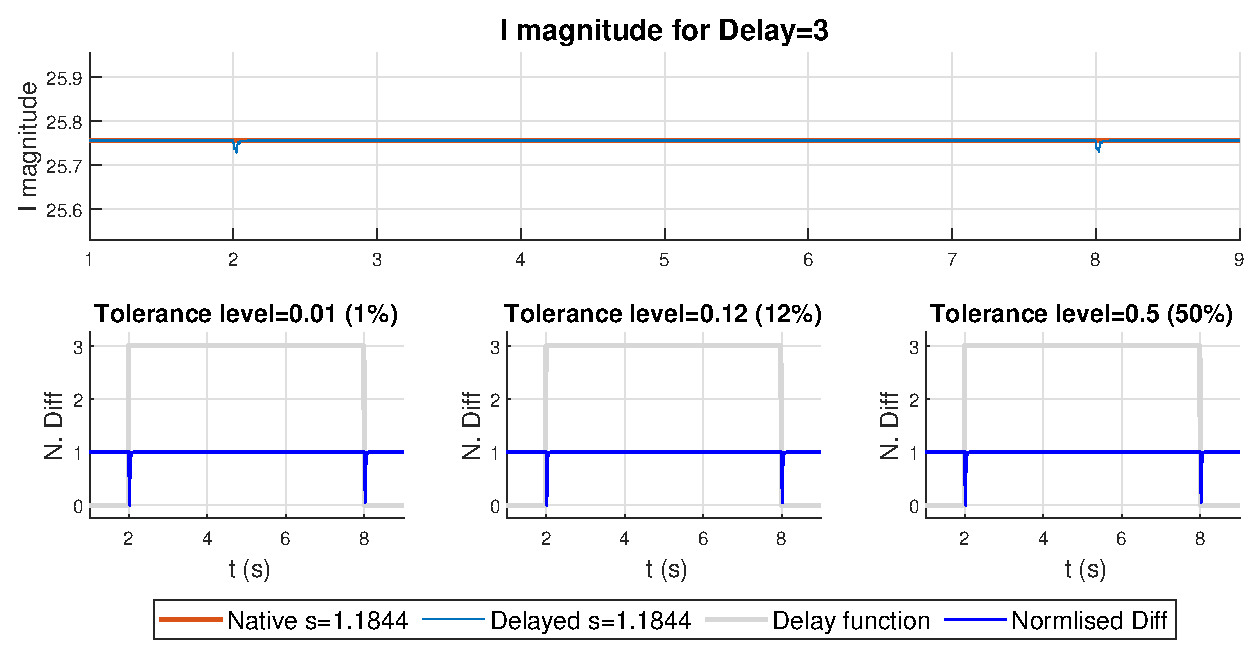
\includegraphics[width=0.95\textwidth]{PMUsim-figures/DelayOf_3/Instant_iMagnitude.eps}} \\ 
   \fbox{     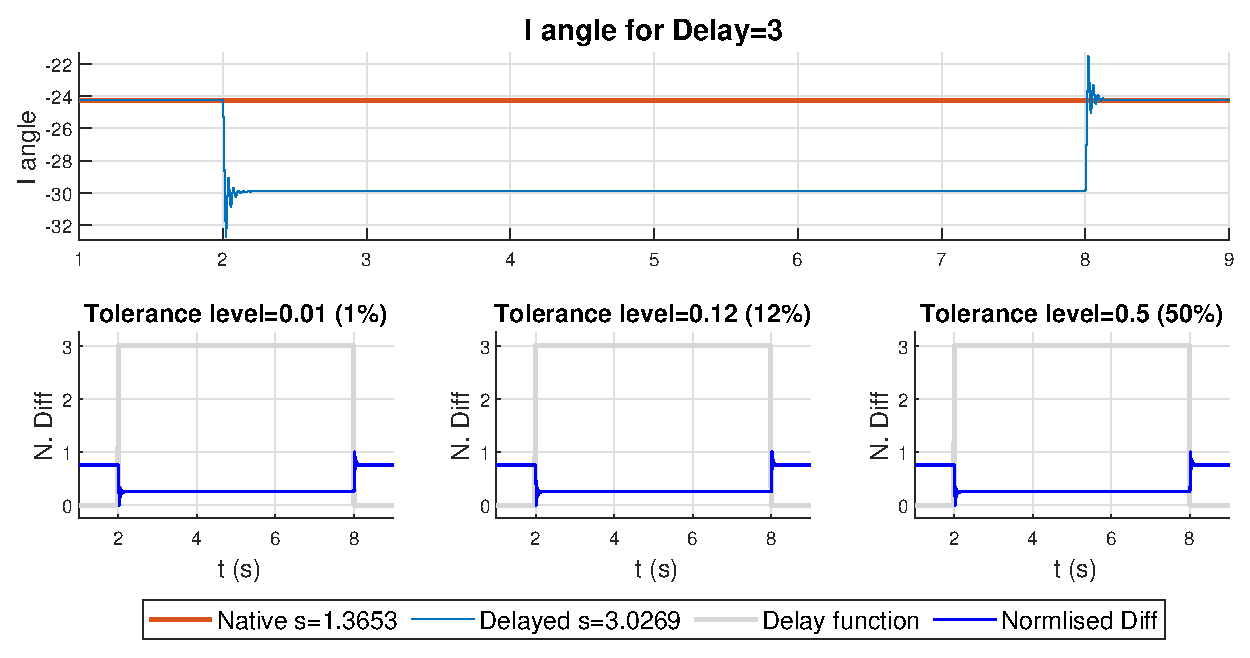
\includegraphics[width=0.95\textwidth]{PMUsim-figures/DelayOf_3/Instant_iAngle.eps}} \\    
   \fbox{    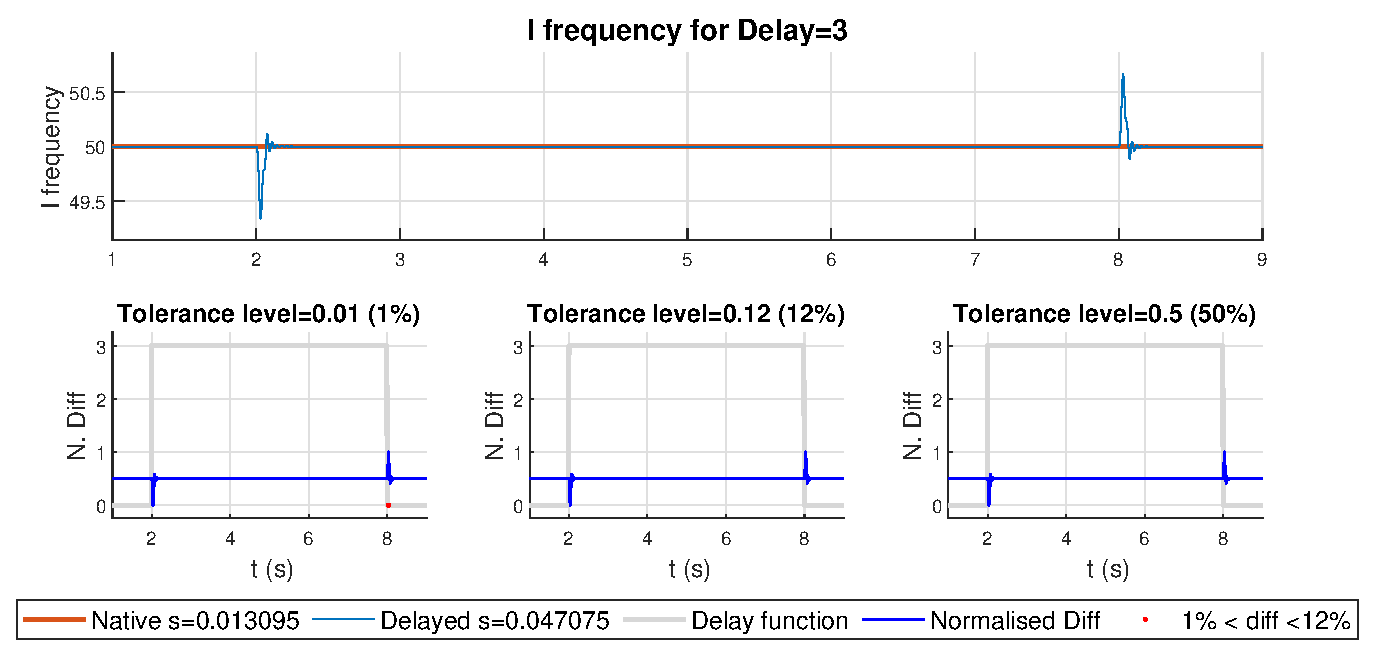
\includegraphics[width=0.95\textwidth]{PMUsim-figures/DelayOf_3/Instant_iFrequency.eps}}


  \end{tabular}
\caption{Results for Impedance Output for Instant Delay equal to Three }
\label{fig:ImpedanceInstantDelayThree}
     \tcbox[size=small, standard jigsaw, opacityback=0, boxrule=0pt,halign=justify]{
     Comments:}{
          \begin{itemize}
         \item      Apparently identical spikes are present for the magnitude graph, at initiation and termination of attack. 
         \item Similar, but mirrored, spikes are apparent for the frequency, whereas the spikes for angle differs.
         \item  A small constant shift of angle, possibly $-10^0$, is apparent, whereas the magnitude and frequency shows no constant alteration of value during the main period of the attack.
          \end{itemize} }
\end{figure}






\newpage
\begin{figure}[H]
\begin{tabular}{c}
  \fbox{  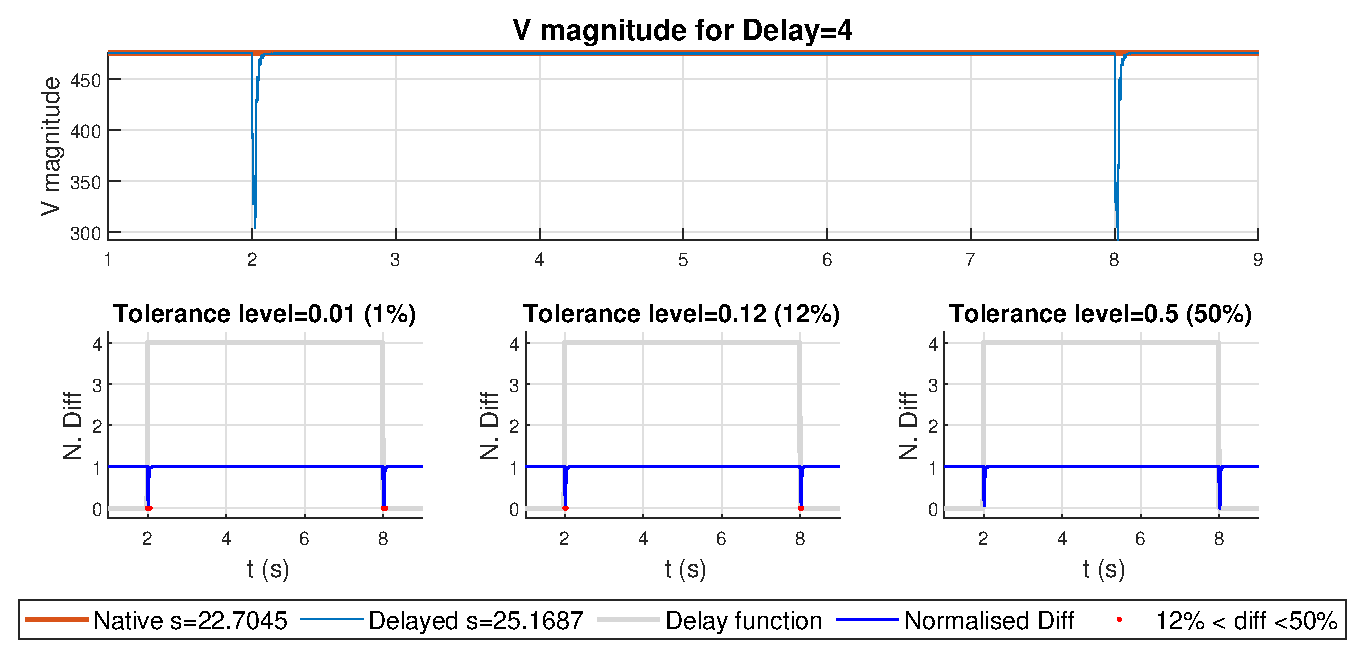
\includegraphics[width=0.95\textwidth]{PMUsim-figures/DelayOf_4/Instant_vMagnitude.eps}} \\ 
  \fbox{     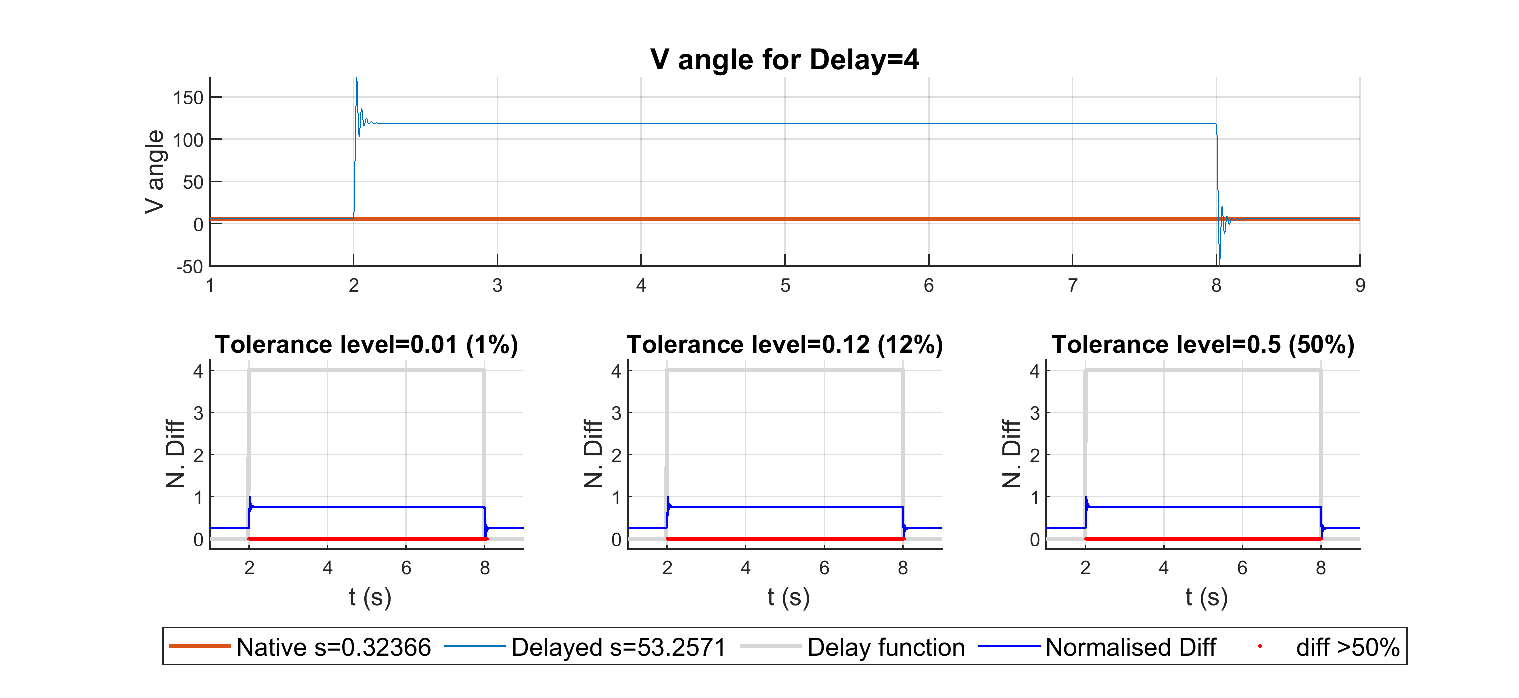
\includegraphics[width=0.95\textwidth]{PMUsim-figures/DelayOf_4/Instant_vAngle.eps}} \\   
   \fbox{    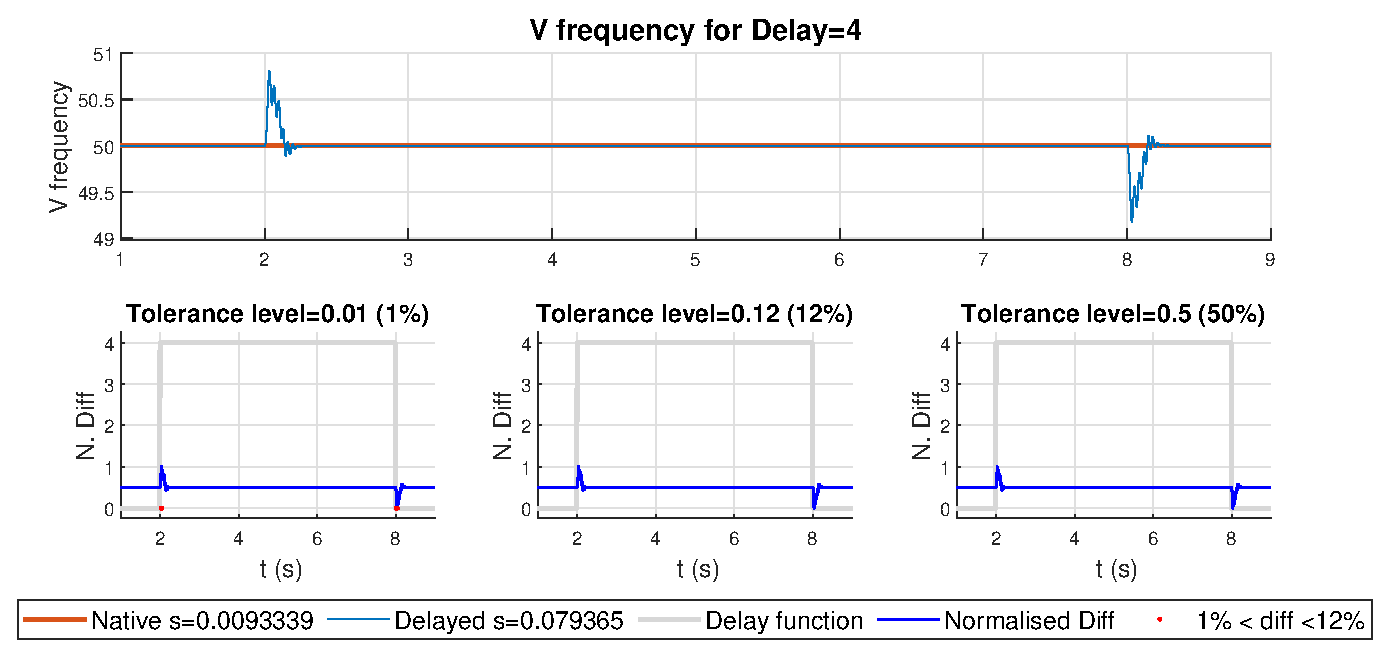
\includegraphics[width=0.95\textwidth]{PMUsim-figures/DelayOf_4/Instant_vFrequency.eps}} 
 
  \end{tabular}
\caption{Results for Voltage Output for Instant Delay equal to Four }
\label{fig:VoltageInstantDelayFour}

     \tcbox[size=small, standard jigsaw, opacityback=0, boxrule=0pt,halign=justify]{
     Comments:}{
          \begin{itemize}
         \item      Apparently identical spikes are present for the magnitude graph, at initiation and termination of attack. 
         \item Similar, but mirrored, spikes are apparent for angle and frequency.
         \item  A constant shift of angle, possibly $120^0$, is apparent, whereas the other components, magnitude and frequency, shows no constant alteration of value.
          \end{itemize} }
\end{figure}

\newpage
\begin{figure}[H]
\begin{tabular}{c}
  \fbox{  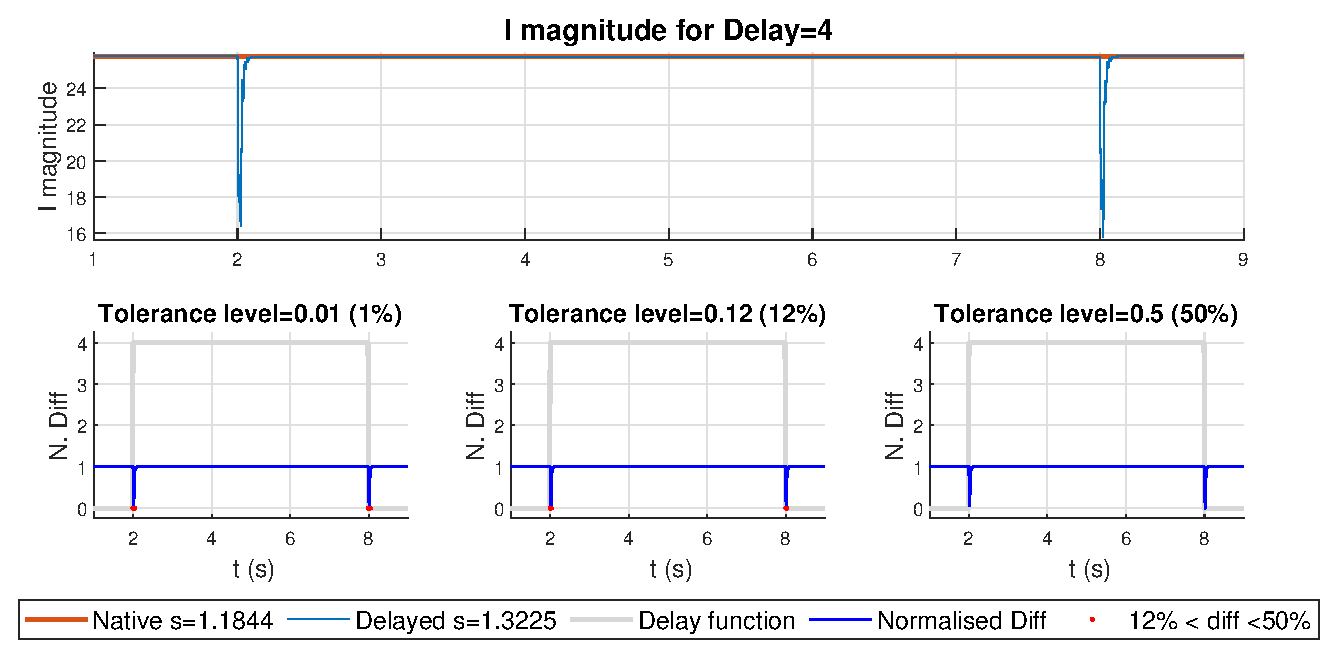
\includegraphics[width=0.95\textwidth]{PMUsim-figures/DelayOf_4/Instant_iMagnitude.eps}} \\ 
   \fbox{     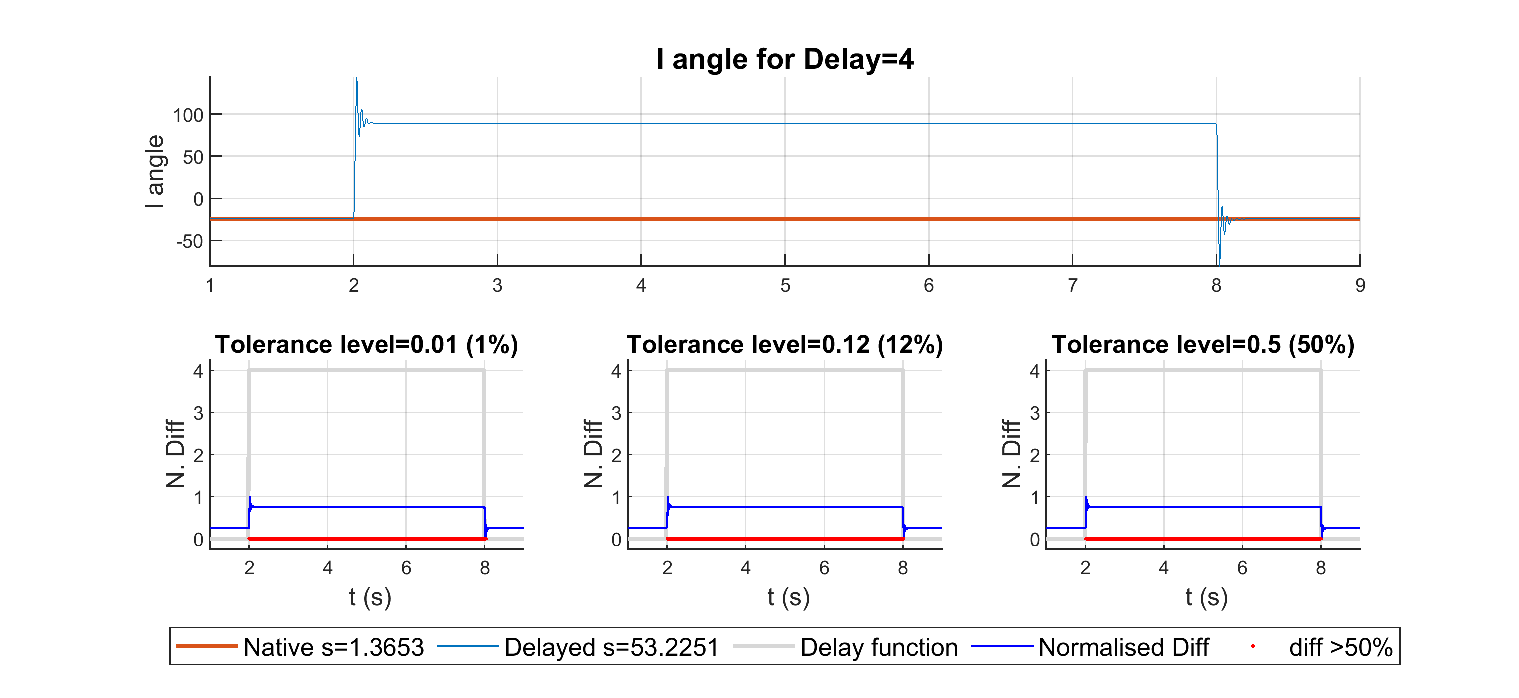
\includegraphics[width=0.95\textwidth]{PMUsim-figures/DelayOf_4/Instant_iAngle.eps}} \\    
   \fbox{    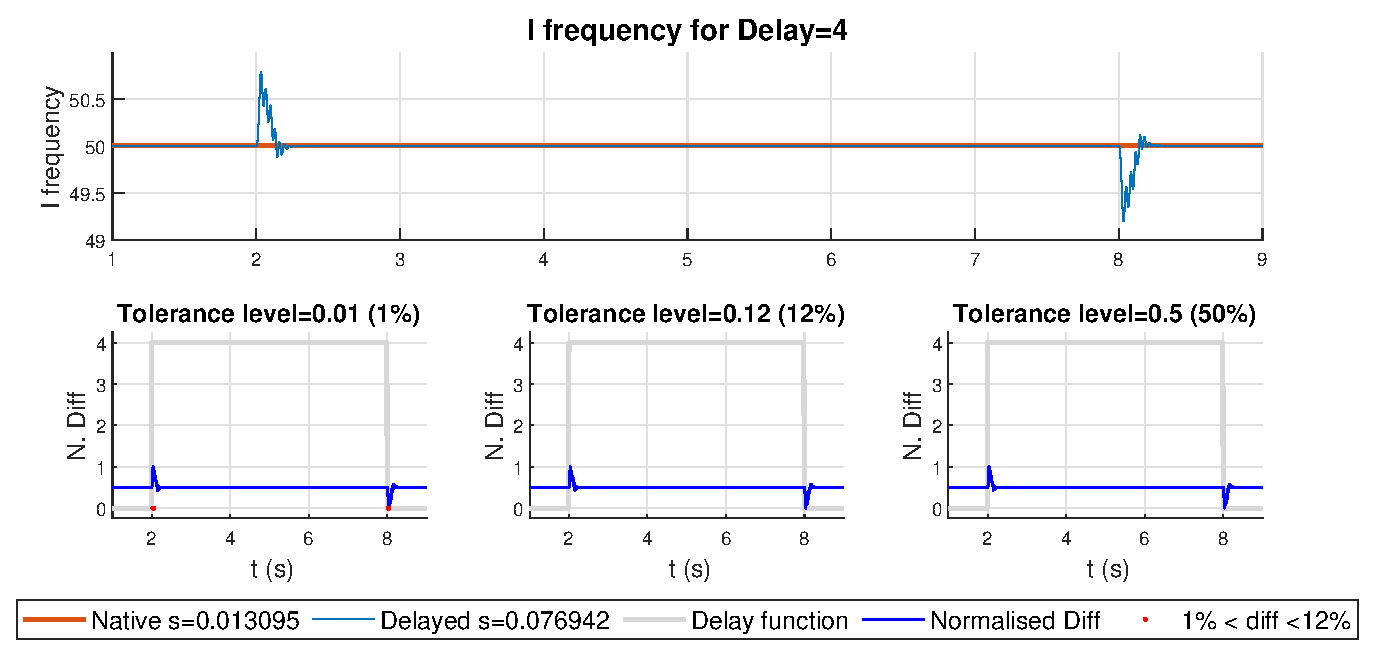
\includegraphics[width=0.95\textwidth]{PMUsim-figures/DelayOf_4/Instant_iFrequency.eps}}


  \end{tabular}
\caption{Results for Impedance Output for Instant Delay equal to Four }
\label{fig:ImpedanceInstantDelayFour}

     \tcbox[size=small, standard jigsaw, opacityback=0, boxrule=0pt,halign=justify]{
     Comments:}{
          \begin{itemize}
         \item      Apparently identical spikes are present for the magnitude graph, at initiation and termination of attack. 
         \item Similar, but mirrored, spikes are apparent for angle and frequency.
         \item  A constant shift of angle, possibly $120^0$, is apparent, whereas the other components, magnitude and frequency, shows no constant alteration of value.
          \end{itemize} }

\end{figure}




\newpage
\begin{figure}[H]
\begin{tabular}{c}
  \fbox{  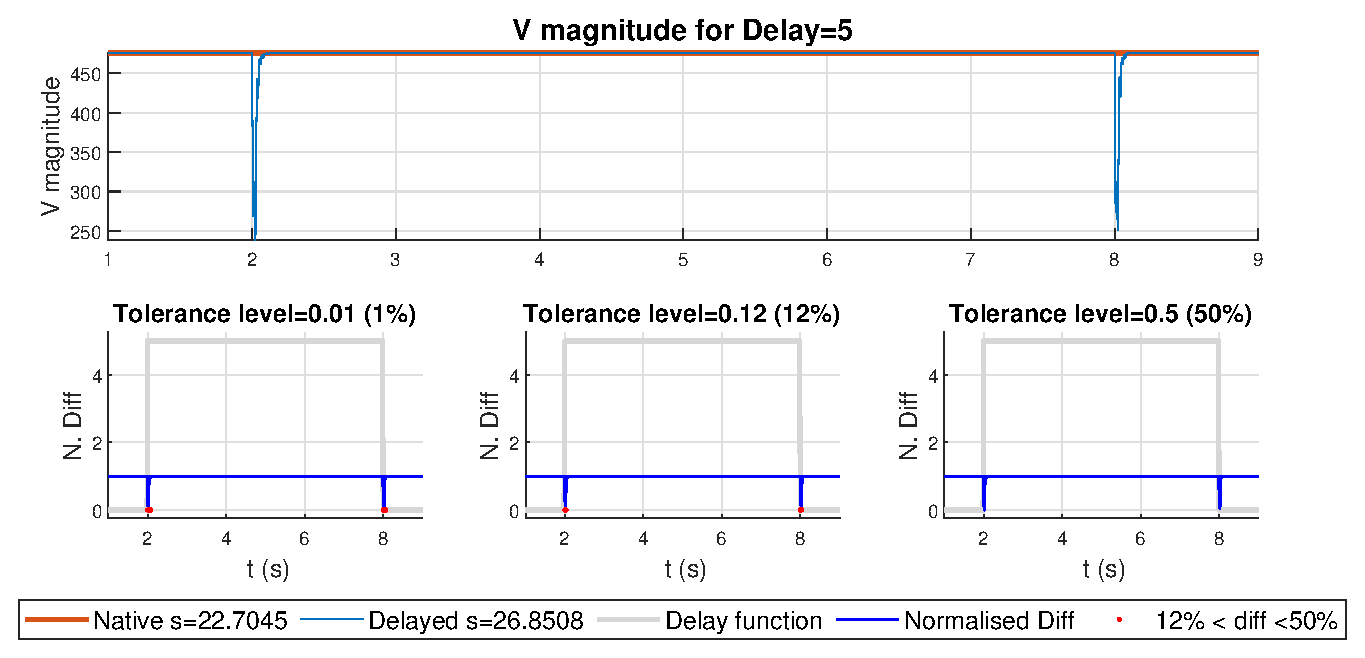
\includegraphics[width=0.95\textwidth]{PMUsim-figures/DelayOf_5/Instant_vMagnitude.eps}} \\ 
    \fbox{     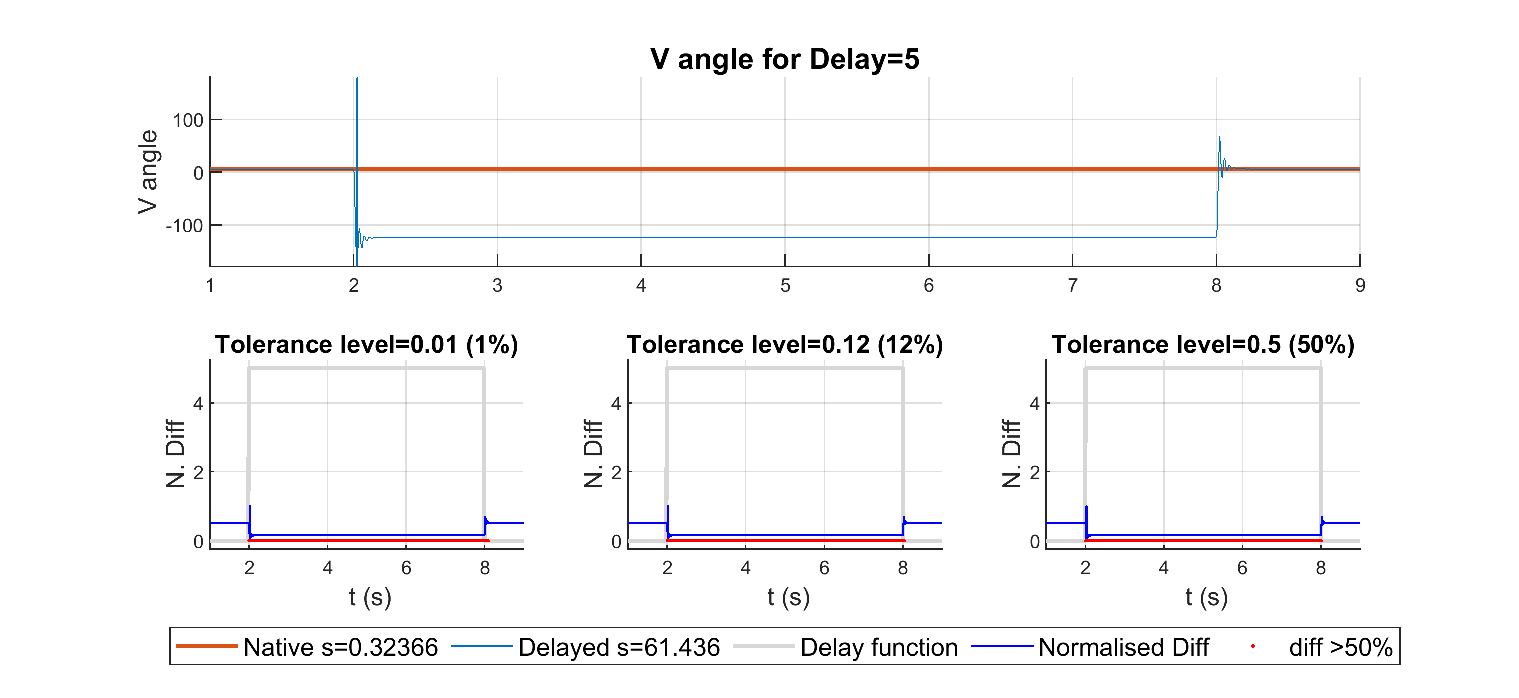
\includegraphics[width=0.95\textwidth]{PMUsim-figures/DelayOf_5/Instant_vAngle.eps}} \\   
   \fbox{    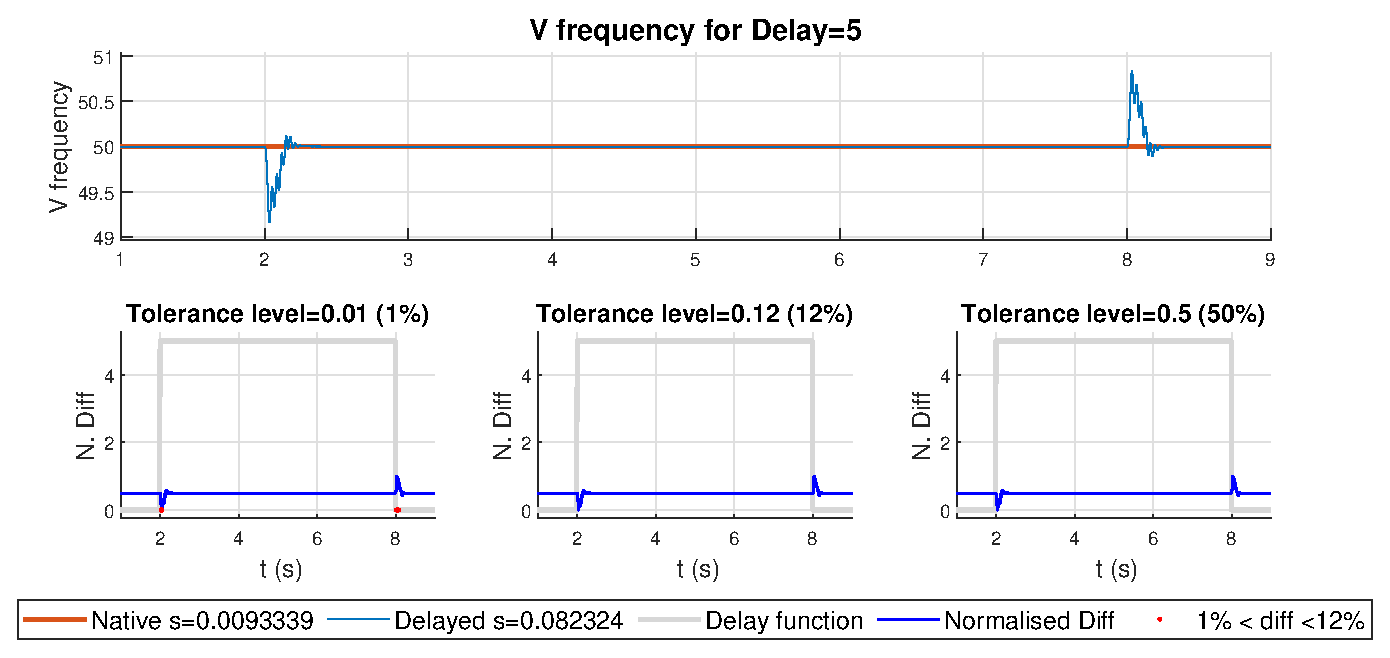
\includegraphics[width=0.95\textwidth]{PMUsim-figures/DelayOf_5/Instant_vFrequency.eps}}


  \end{tabular}
\caption{Results for Voltage Output for Instant Delay equal to Five }
\label{fig:VoltageInstantDelayFive}
     \tcbox[size=small, standard jigsaw, opacityback=0, boxrule=0pt,halign=justify]{
     Comments:}{
          \begin{itemize}
         \item      Apparently identical spikes are present for the magnitude graph, at initiation and termination of attack. 
         \item Similar, but mirrored, spikes are apparent for the frequency, whereas the spikes for angle differs.
         \item  A constant shift of angle, possibly $-120^0$, is apparent, whereas the magnitude and frequency shows no constant alteration of value during the main period of the attack.
          \end{itemize} }
\end{figure}
\newpage
\begin{figure}[H]
\begin{tabular}{c}
  \fbox{  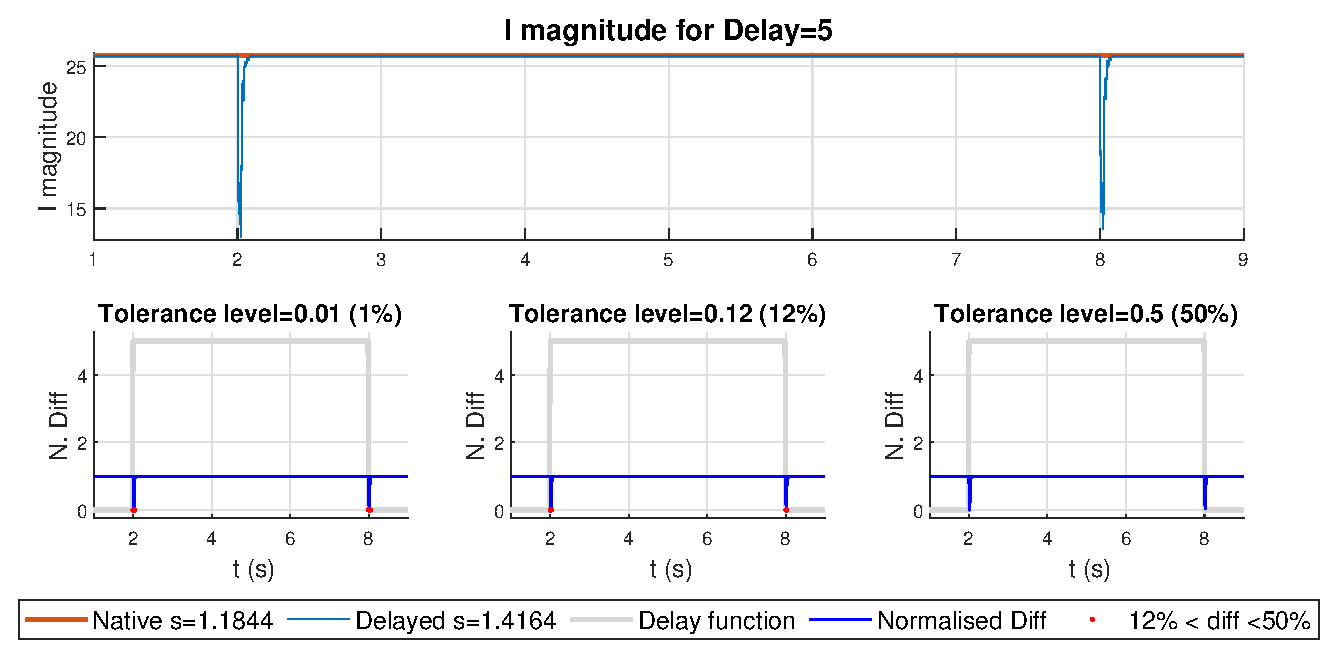
\includegraphics[width=0.95\textwidth]{PMUsim-figures/DelayOf_5/Instant_iMagnitude.eps}} \\ 
    \fbox{     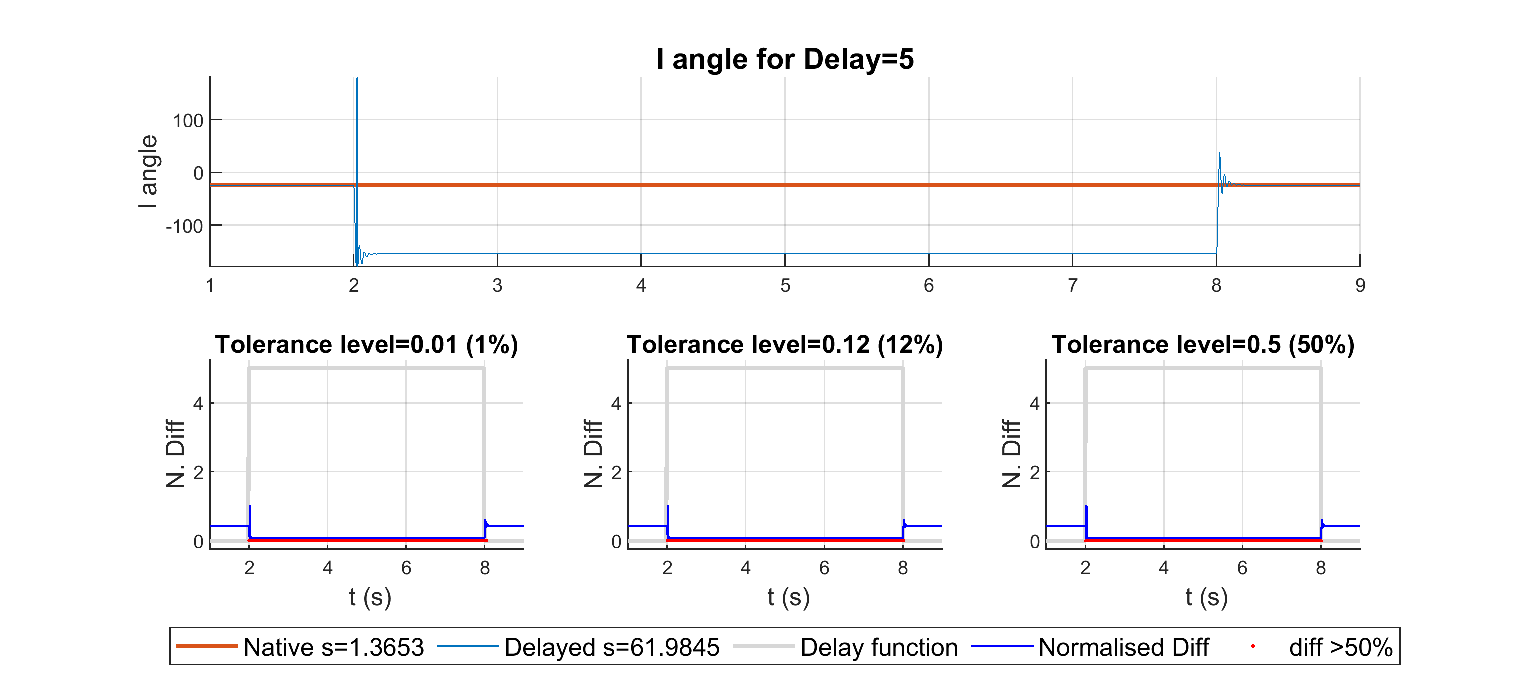
\includegraphics[width=0.95\textwidth]{PMUsim-figures/DelayOf_5/Instant_iAngle.eps}} \\  
   \fbox{    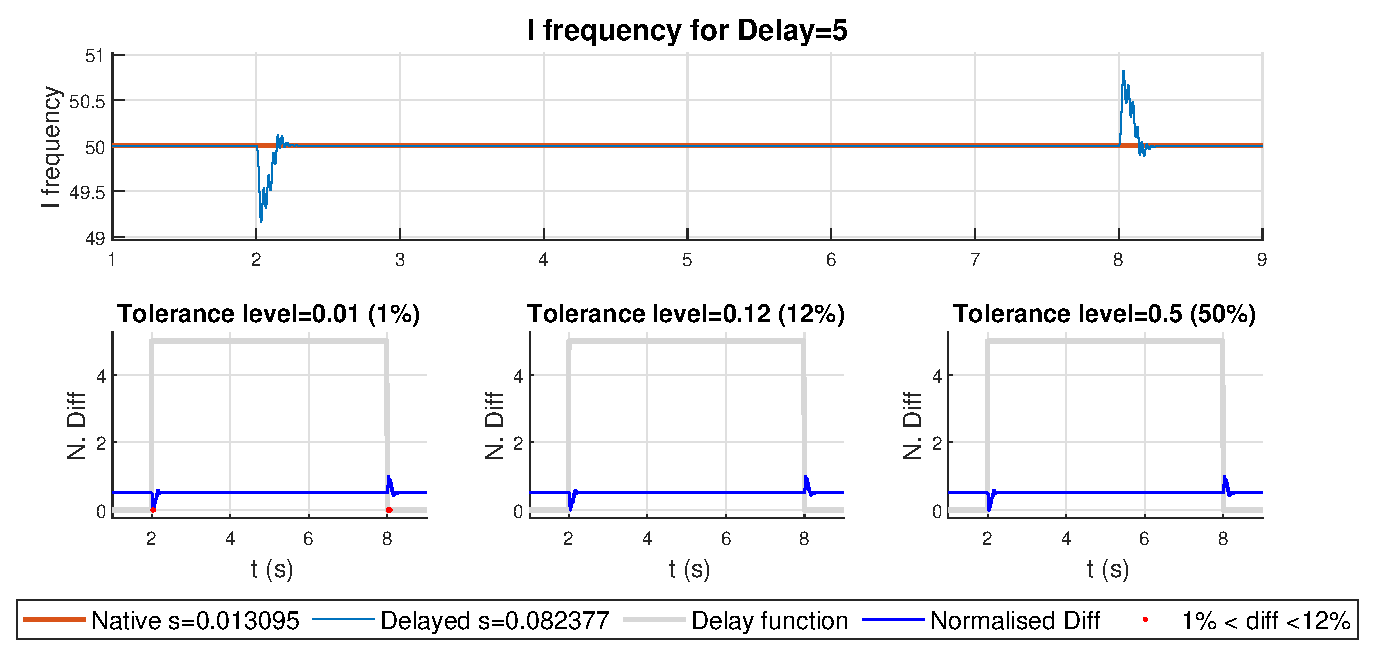
\includegraphics[width=0.95\textwidth]{PMUsim-figures/DelayOf_5/Instant_iFrequency.eps}}

 
  \end{tabular}
\caption{Results for Impedance Output for Instant Delay equal to Five }
\label{fig:ImpedanceInstantDelayFive}

     \tcbox[size=small, standard jigsaw, opacityback=0, boxrule=0pt,halign=justify]{
     Comments:}{
          \begin{itemize}
         \item      Apparently identical spikes are present for the magnitude graph, at initiation and termination of attack. 
         \item Similar, but mirrored, spikes are apparent for the frequency, whereas the spikes for angle differs.
         \item  A constant shift of angle, possibly $-120^0$, is apparent, whereas the magnitude and frequency shows no constant alteration of value during the main period of the attack.
         \end{itemize} }

\end{figure}


\newpage
\begin{figure}[H]
\begin{tabular}{c}
  \fbox{  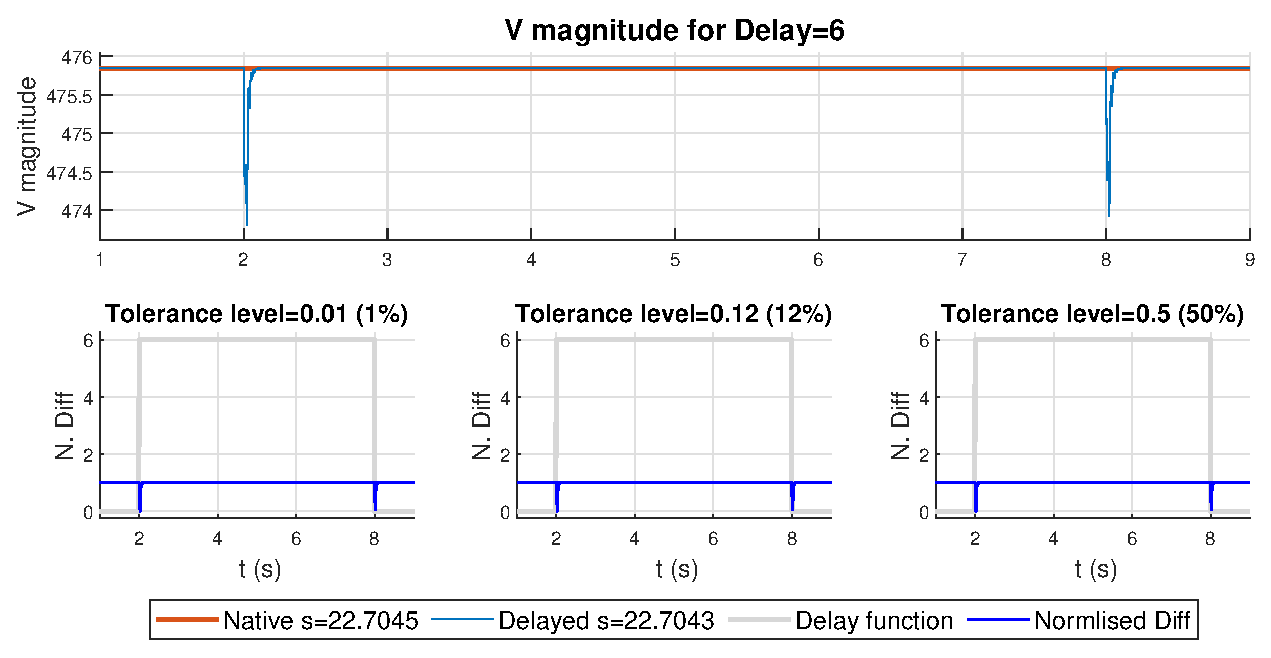
\includegraphics[width=0.95\textwidth]{PMUsim-figures/DelayOf_6/Instant_vMagnitude.eps}} \\ 
   \fbox{     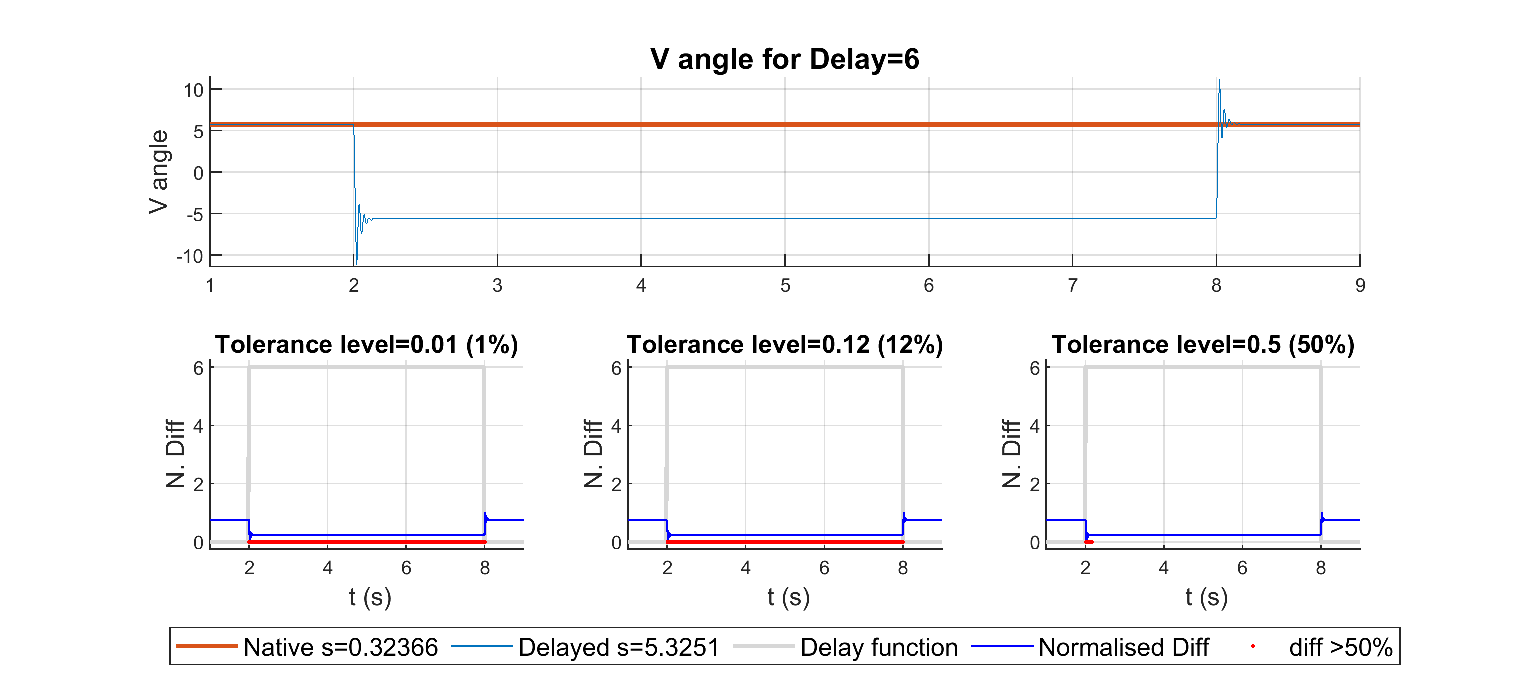
\includegraphics[width=0.95\textwidth]{PMUsim-figures/DelayOf_6/Instant_vAngle.eps}} \\   
   \fbox{    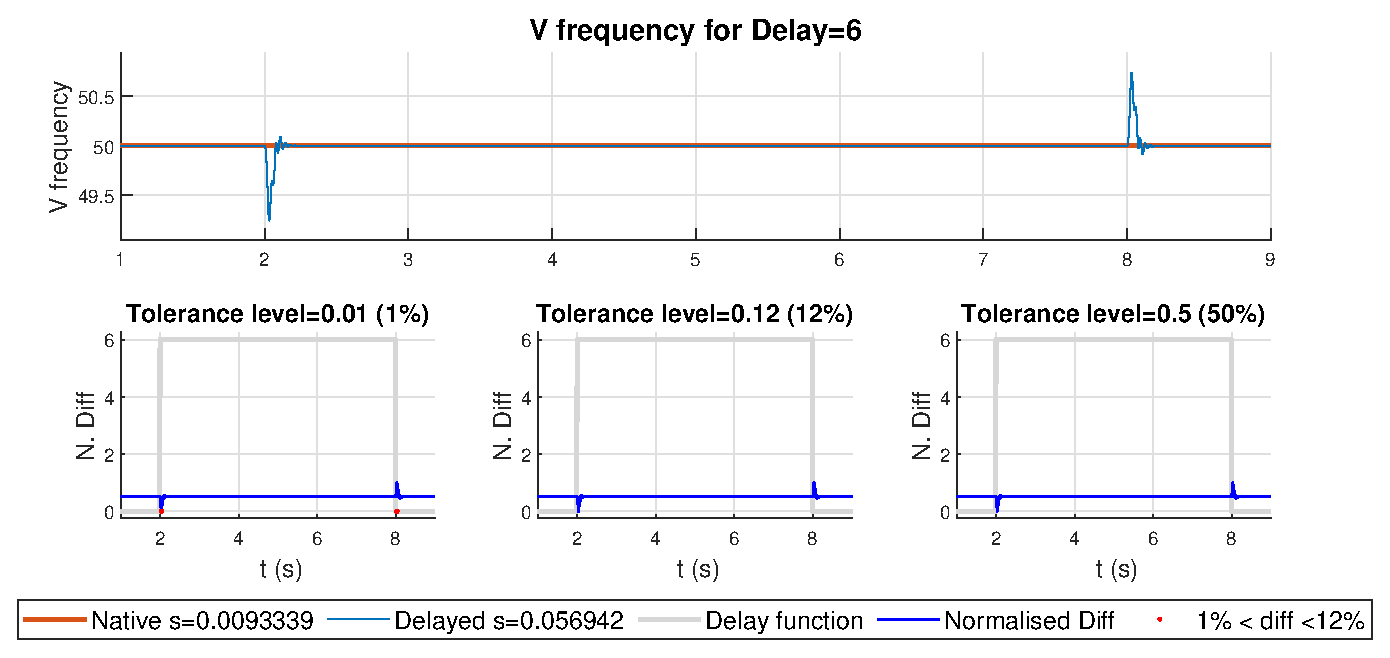
\includegraphics[width=0.95\textwidth]{PMUsim-figures/DelayOf_6/Instant_vFrequency.eps}}

 
  \end{tabular}
\caption{Results for Voltage Output for Instant Delay equal to Six }
\label{fig:VoltageInstantDelaySix}
     \tcbox[size=small, standard jigsaw, opacityback=0, boxrule=0pt,halign=justify]{
     Comments:}{
          \begin{itemize}
         \item      Apparently identical spikes are present for the magnitude graph, at initiation and termination of attack. 
         \item Similar, but mirrored, spikes are apparent for the frequency, whereas the spikes for angle differs.
         \item  A small constant shift of angle, possibly $-6^0$, is apparent, whereas the magnitude and frequency shows no constant alteration of value during the main period of the attack.
          \end{itemize} }
		  \end{figure}
\newpage
\begin{figure}[H]
\begin{tabular}{c}
  \fbox{  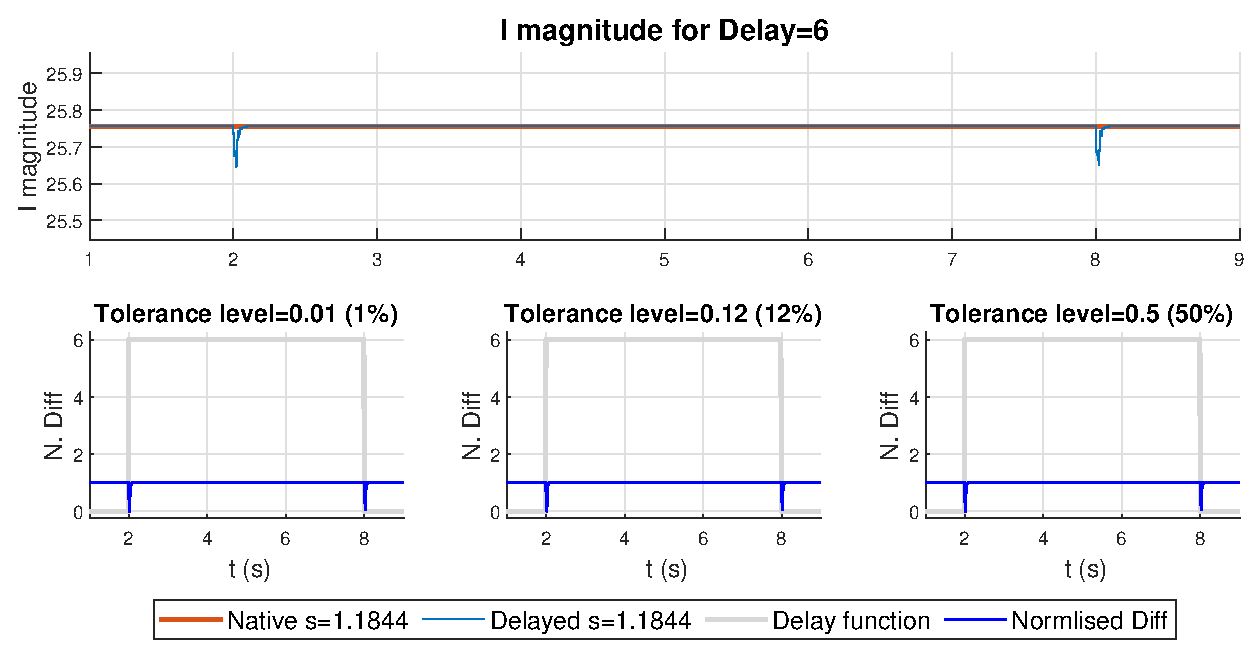
\includegraphics[width=0.95\textwidth]{PMUsim-figures/DelayOf_6/Instant_iMagnitude.eps}} \\ 
   \fbox{     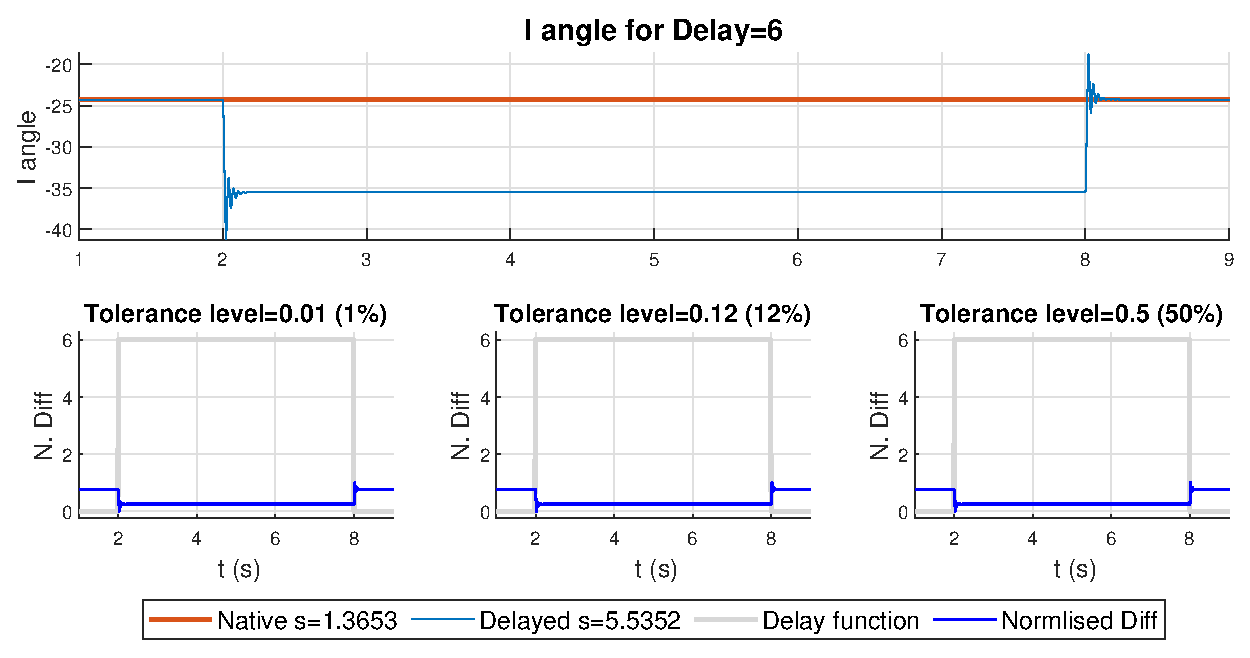
\includegraphics[width=0.95\textwidth]{PMUsim-figures/DelayOf_6/Instant_iAngle.eps}} \\   
   \fbox{    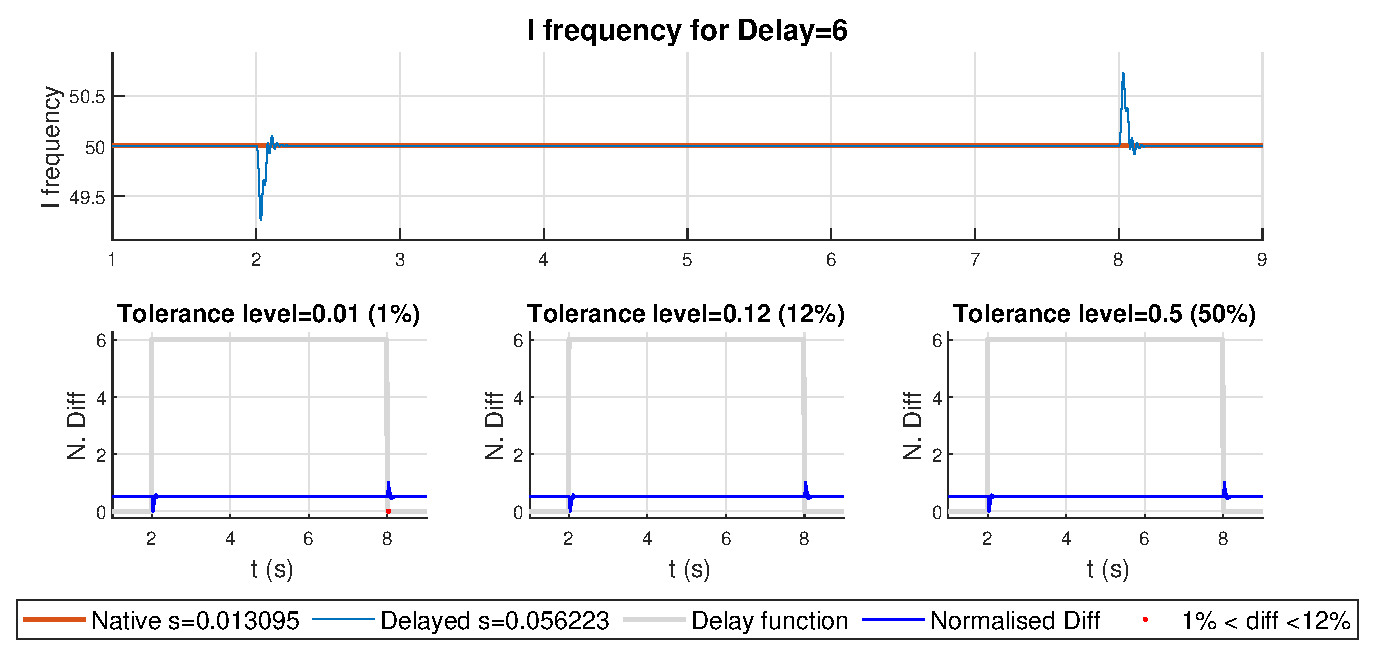
\includegraphics[width=0.95\textwidth]{PMUsim-figures/DelayOf_6/Instant_iFrequency.eps}}

 
  \end{tabular}
\caption{Results for Impedance Output for Instant Delay equal to Six }
\label{fig:ImpedanceInstantDelaySix}
     \tcbox[size=small, standard jigsaw, opacityback=0, boxrule=0pt,halign=justify]{
     Comments:}{
          \begin{itemize}
         \item      Apparently identical spikes are present for the magnitude graph, at initiation and termination of attack. 
         \item Similar, but mirrored, spikes are apparent for the frequency, whereas the spikes for angle differs.
         \item  A small constant shift of angle, possibly $-6^0$, is apparent, whereas the magnitude and frequency shows no constant alteration of value during the main period of the attack.
          \end{itemize} }
		  \end{figure}

\newpage
\subsection{Conclusive remarks on instant delay simulations}


\subsubsection{Instant Delay Level of One}
Figures \ref{fig:VoltageInstantDelayOne} and \ref{fig:ImpedanceInstantDelayOne} shows the result of the Instant delay attack of level One. 

\subsubsection{Instant Delay Level of Two}
Figures \ref{fig:VoltageInstantDelayTwo} and \ref{fig:ImpedanceInstantDelayTwo} shows the result of the Instant delay attack of level Two. 

\subsubsection{Instant Delay Level of Three}
Figures \ref{fig:VoltageInstantDelayThree} and \ref{fig:ImpedanceInstantDelayThree} shows the result of the Instant delay attack of level Three. 

\subsubsection{Instant Delay Level of Four}
Figures \ref{fig:VoltageInstantDelayFour} and \ref{fig:ImpedanceInstantDelayFour} shows the result of the Instant delay attack of level Four. 

\subsubsection{Instant Delay Level of Five}
Figures \ref{fig:VoltageInstantDelayFive} and \ref{fig:ImpedanceInstantDelayFive} shows the result of the Instant delay attack of level Five. 

\subsubsection{Instant Delay Level of Six}
Figures \ref{fig:VoltageInstantDelaySix} and \ref{fig:ImpedanceInstantDelaySix} shows the result of the Instant delay attack of level Six. 








\newpage
\section{Step-Wise Delay functions}
The other flavour of delay attack considered, the step-Wise delay attack, focuses on effects caused by a slower rise of the delay level towards a pre-determined target level of delay. As there are no step-wise attack for delay level one, this category of attacks initiates the sequence of attacks by starting with a delay level of two.

The attack focuses on the following 
\begin{itemize}
\item What are the effects of repetitive increases of the delay level by one for different number of repetitions?
\item Are there any patterns observable:
\begin{itemize}
    \item Do the termination of the attack cancel the effect of the attack
    \item Do the next level of increase produce corresponding effects? 
\end{itemize}

\end{itemize}



On a suitable number of next pages, the the figures showing the results of running the Step-wise Delay Simulations of levels One trough Six are available for inspection of the results. \\ 
Comments are located underneath each figure.


















\newpage
\begin{figure}[H]
\begin{tabular}{c}
  \fbox{  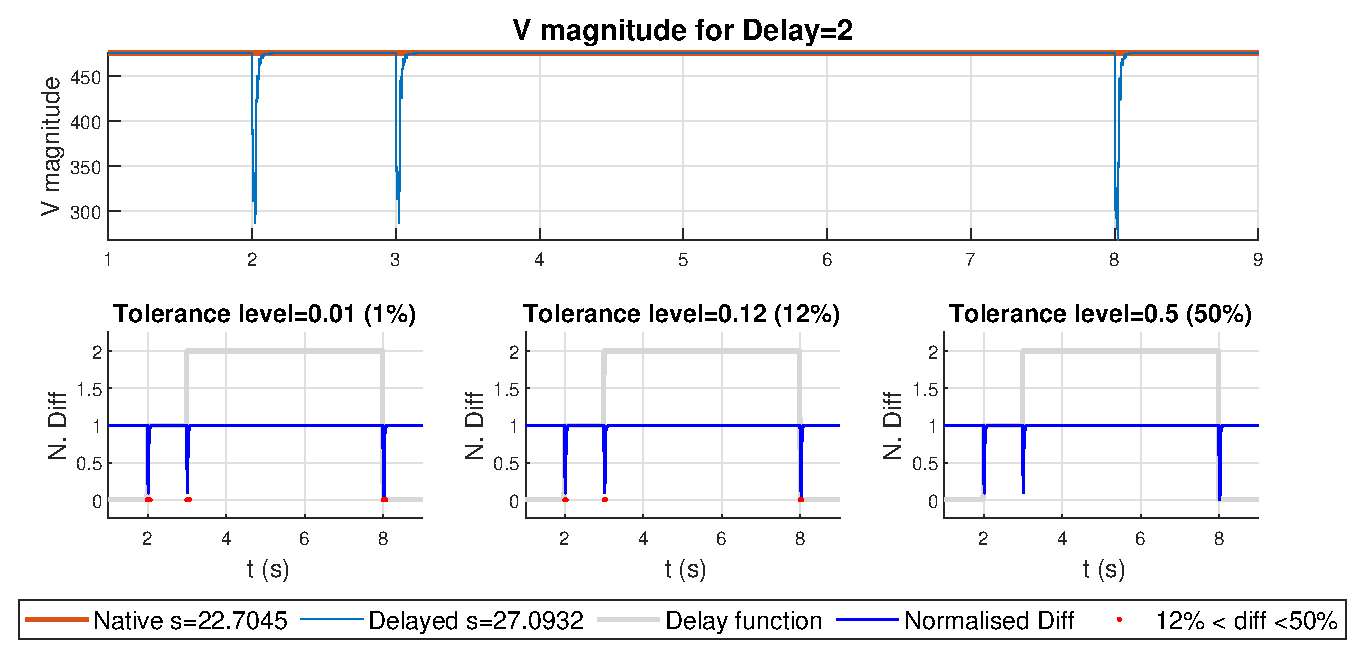
\includegraphics[width=0.95\textwidth]{PMUsim-figures/DelayOf_2/Step_vMagnitude.eps}} \\ 
    \fbox{     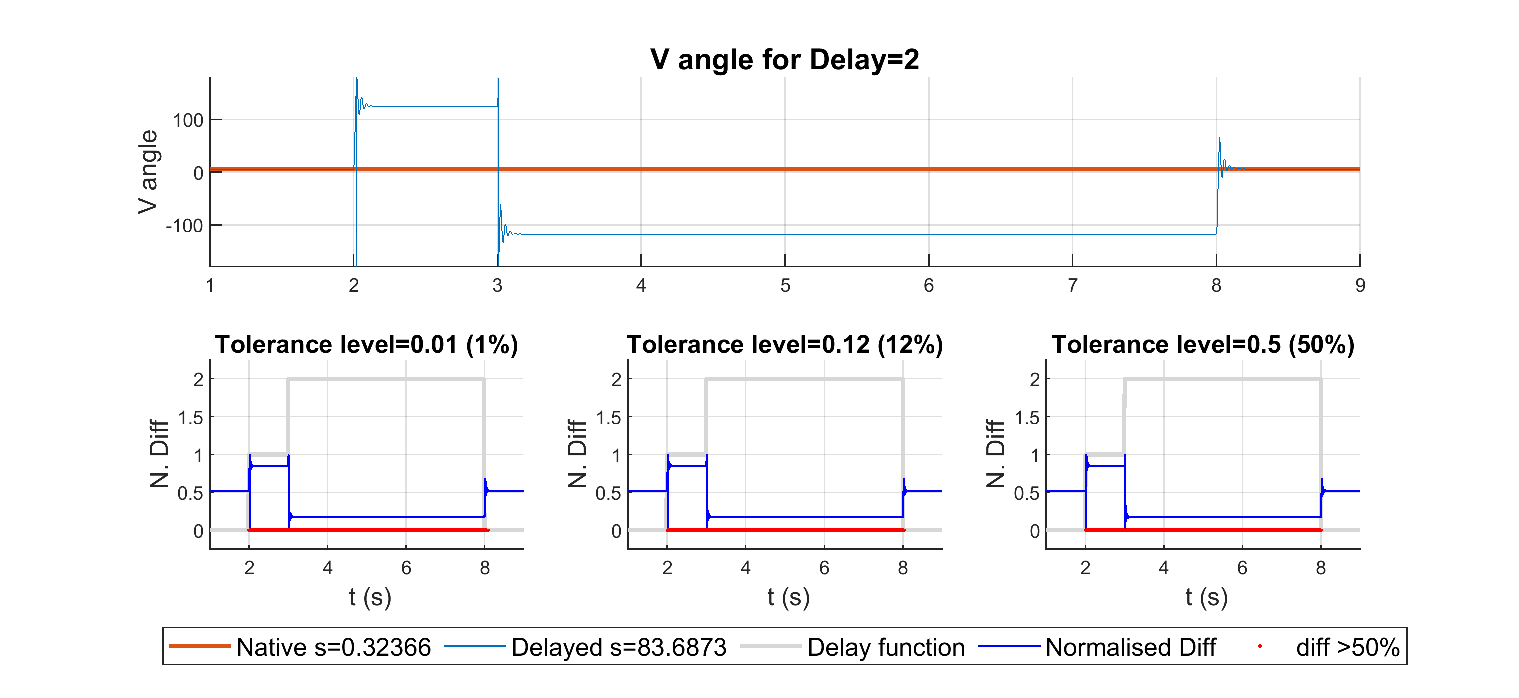
\includegraphics[width=0.95\textwidth]{PMUsim-figures/DelayOf_2/Step_vAngle.eps}} \\ 
  
   \fbox{    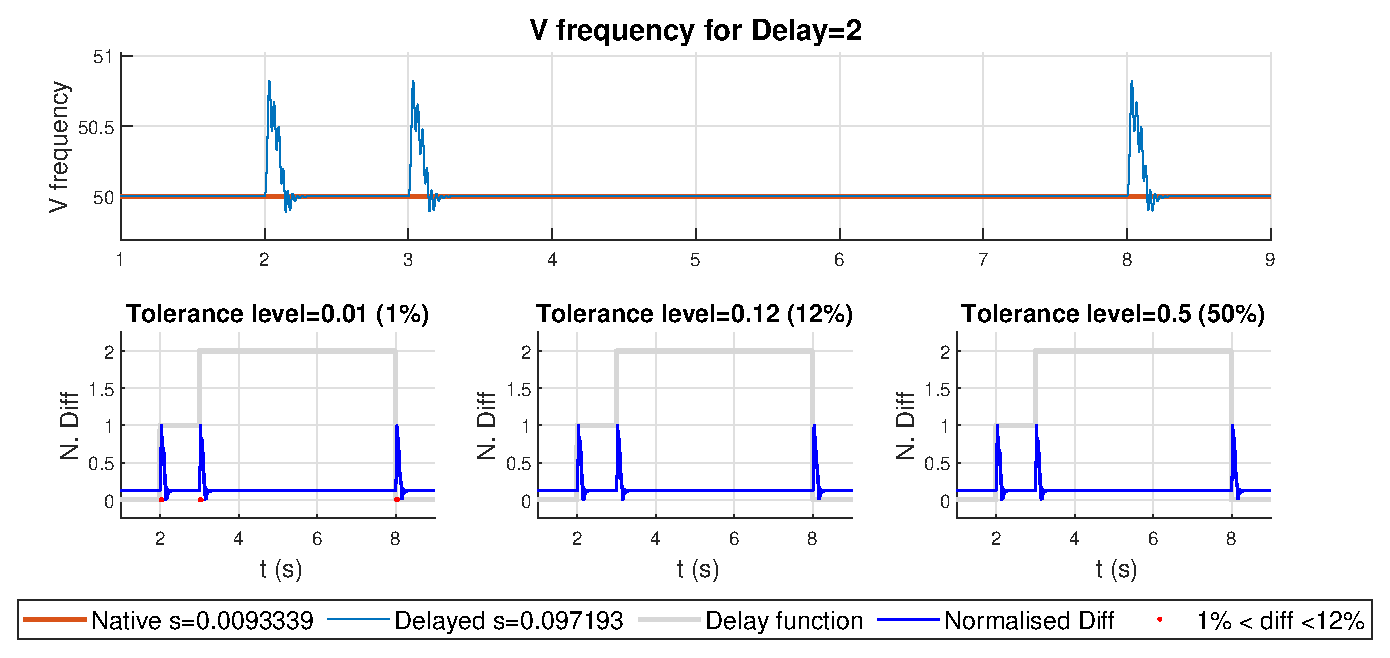
\includegraphics[width=0.95\textwidth]{PMUsim-figures/DelayOf_2/Step_vFrequency.eps}}


  \end{tabular}
\caption{Results for Voltage Output for Step-Wise Delay equal to Two }
\label{fig:VoltageStepWiseDelayTwo}
     \tcbox[size=small, standard jigsaw, opacityback=0, boxrule=0pt,halign=justify]{
     Comments:}{
          \begin{itemize}
         \item     The component graphs shows combinations of the results for the instant delay simulations of levels one and two. 
          \end{itemize} }

\end{figure}


\newpage
\begin{figure}[H]
\begin{tabular}{c}
  \fbox{  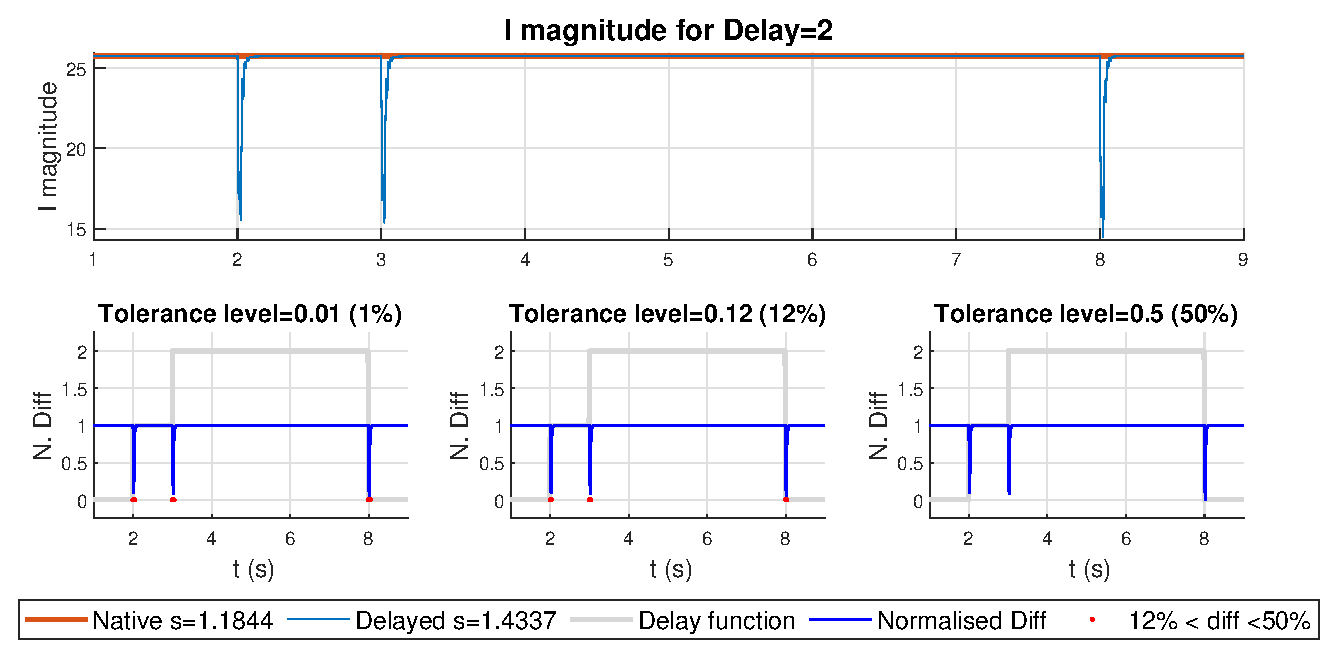
\includegraphics[width=0.95\textwidth]{PMUsim-figures/DelayOf_2/Step_iMagnitude.eps}} \\ 
   \fbox{     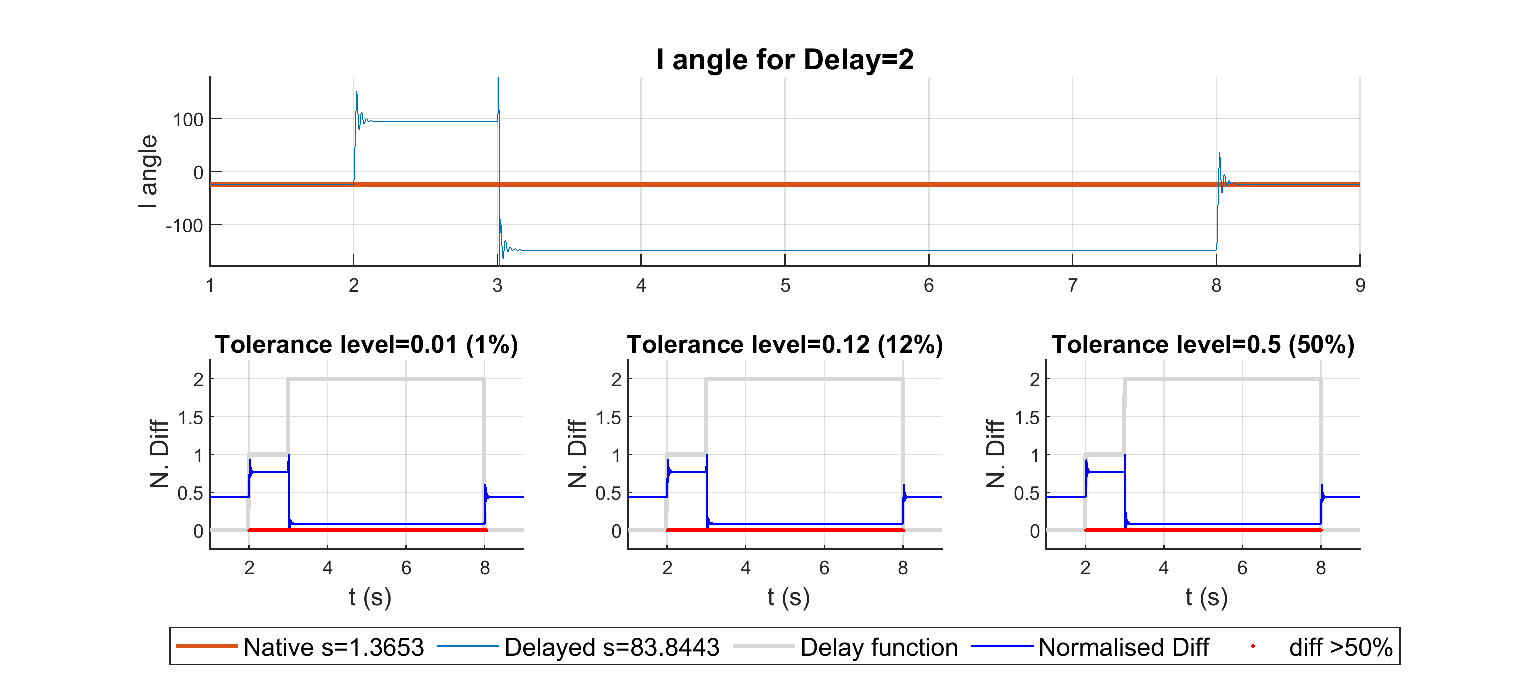
\includegraphics[width=0.95\textwidth]{PMUsim-figures/DelayOf_2/Step_iAngle.eps}} \\   
   \fbox{    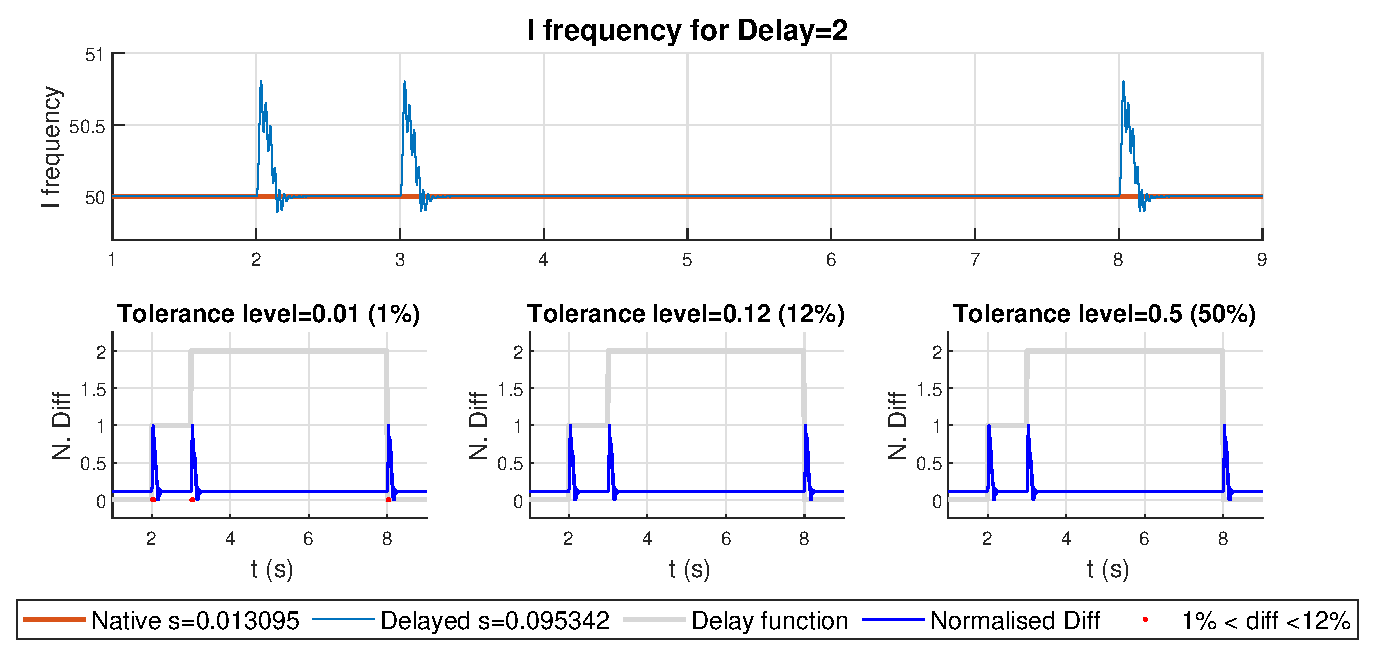
\includegraphics[width=0.95\textwidth]{PMUsim-figures/DelayOf_2/Step_iFrequency.eps}} 


  \end{tabular}
\caption{Results for Impedance Output for Step-Wise Delay equal to Two }
\label{fig:ImpedanceStepWiseDelayTwo}
     \tcbox[size=small, standard jigsaw, opacityback=0, boxrule=0pt,halign=justify]{
     Comments:}{
          \begin{itemize}
         \item     The component graphs shows combinations of the results for the instant delay simulations of levels one and two. 
          \end{itemize} }

\end{figure}





\newpage
\begin{figure}[H]
\begin{tabular}{c}
  \fbox{  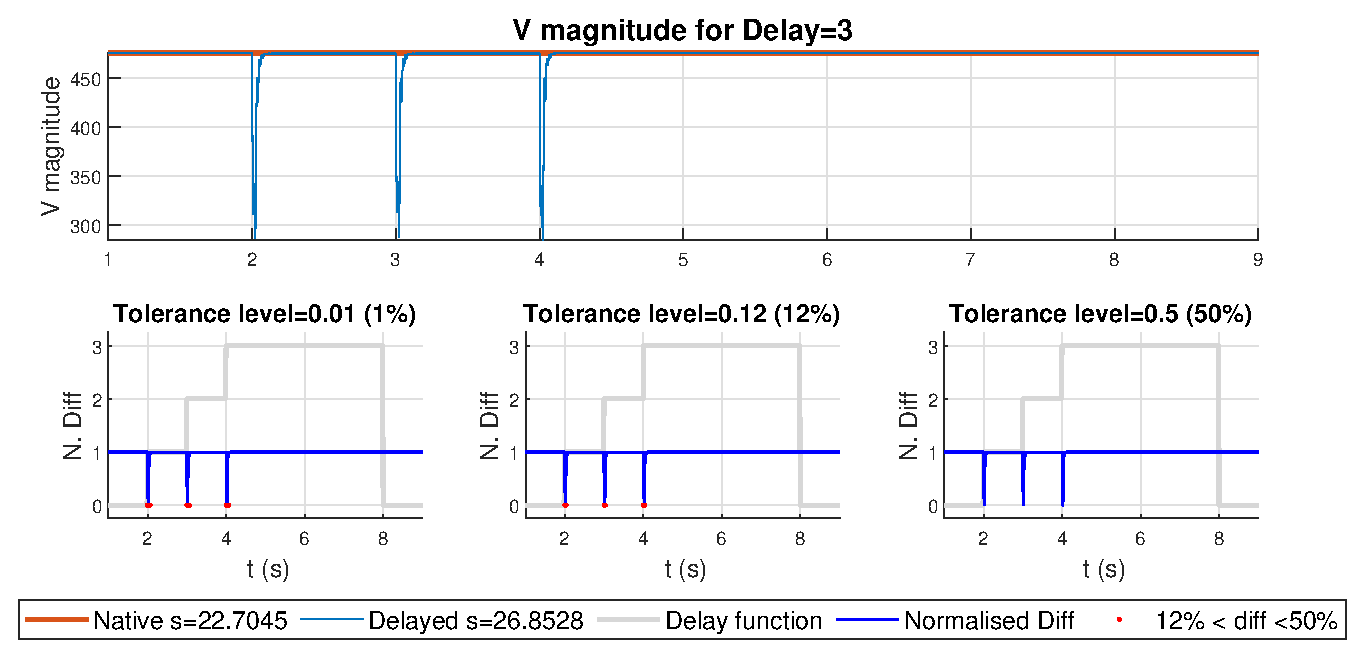
\includegraphics[width=0.95\textwidth]{PMUsim-figures/DelayOf_3/Step_vMagnitude.eps}} \\ 
   \fbox{     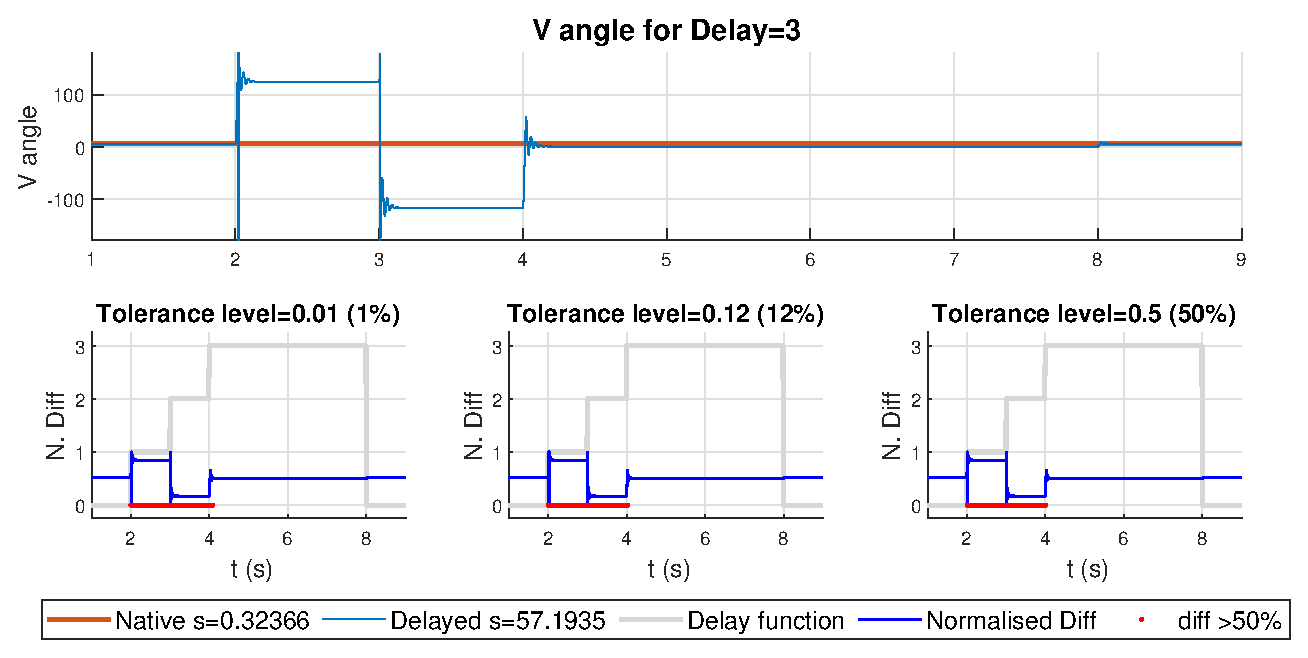
\includegraphics[width=0.95\textwidth]{PMUsim-figures/DelayOf_3/Step_vAngle.eps}} \\    
   \fbox{    \includegraphics[width=0.95\textwidth]{PMUsim-figures/DelayOf_3/Step_vFrequency.eps}}

  \end{tabular}
\caption{Results for Voltage Output for Step-Wise Delay equal to Three }
\label{fig:VoltageStepWiseDelayThree}
     \tcbox[size=small, standard jigsaw, opacityback=0, boxrule=0pt,halign=justify]{
     Comments:}{
          \begin{itemize}
         \item     The component graphs shows combinations of the results for the instant delay simulations of levels between one and three. 
          \end{itemize} }

\end{figure}

\newpage
\begin{figure}[H]
\begin{tabular}{c}
  \fbox{  \includegraphics[width=0.95\textwidth]{PMUsim-figures/DelayOf_3/Step_iMagnitude.eps}} \\ 
   \fbox{     \includegraphics[width=0.95\textwidth]{PMUsim-figures/DelayOf_3/Step_iAngle.eps}} \\  
   \fbox{    \includegraphics[width=0.95\textwidth]{PMUsim-figures/DelayOf_3/Step_iFrequency.eps}}

    

  \end{tabular}
\caption{Results for Impedance Output for Step-Wise Delay equal to Three }
\label{fig:ImpedanceStepWiseDelayThree}
     \tcbox[size=small, standard jigsaw, opacityback=0, boxrule=0pt,halign=justify]{
     Comments:}{
          \begin{itemize}
         \item     The component graphs shows combinations of the results for the instant delay simulations of levels between one and three. 
          \end{itemize} }

\end{figure}






\newpage
\begin{figure}[H]
\begin{tabular}{c}
  \fbox{  \includegraphics[width=0.95\textwidth]{PMUsim-figures/DelayOf_4/Step_vMagnitude.eps}} \\ 
   \fbox{     \includegraphics[width=0.95\textwidth]{PMUsim-figures/DelayOf_4/Step_vAngle.eps}} \\    
   \fbox{    \includegraphics[width=0.95\textwidth]{PMUsim-figures/DelayOf_4/Step_vFrequency.eps}}


  \end{tabular}
\caption{Results for Voltage Output for Step-Wise Delay equal to Four }
\label{fig:VoltageStepWiseDelayFour}
     \tcbox[size=small, standard jigsaw, opacityback=0, boxrule=0pt,halign=justify]{
     Comments:}{
          \begin{itemize}
         \item     The component graphs shows combinations of the results for the instant delay simulations of levels between one and four. 
          \end{itemize} }

\end{figure}

\newpage
\begin{figure}[H]
\begin{tabular}{c}
  \fbox{  \includegraphics[width=0.95\textwidth]{PMUsim-figures/DelayOf_4/Step_iMagnitude.eps}} \\ 
    \fbox{     \includegraphics[width=0.95\textwidth]{PMUsim-figures/DelayOf_4/Step_iAngle.eps}}  \\  
   \fbox{    \includegraphics[width=0.95\textwidth]{PMUsim-figures/DelayOf_4/Step_iFrequency.eps}} 


  \end{tabular}
\caption{Results for Impedance Output for Step-Wise Delay equal to Four }
\label{fig:ImpedanceStepWiseDelayFour}
     \tcbox[size=small, standard jigsaw, opacityback=0, boxrule=0pt,halign=justify]{
     Comments:}{
          \begin{itemize}
         \item     The component graphs shows combinations of the results for the instant delay simulations of levels between one and four. 
          \end{itemize} }

\end{figure}




\newpage
\begin{figure}[H]
\begin{tabular}{c}
  \fbox{  \includegraphics[width=0.95\textwidth]{PMUsim-figures/DelayOf_5/Step_vMagnitude.eps}} \\ 
  \fbox{     \includegraphics[width=0.95\textwidth]{PMUsim-figures/DelayOf_5/Step_vAngle.eps}} \\    
   \fbox{    \includegraphics[width=0.95\textwidth]{PMUsim-figures/DelayOf_5/Step_vFrequency.eps}}

 
  \end{tabular}
\caption{Results for Voltage Output for Step-Wise Delay equal to Five }
\label{fig:VoltageStepWiseDelayFive}
     \tcbox[size=small, standard jigsaw, opacityback=0, boxrule=0pt,halign=justify]{
     Comments:}{
          \begin{itemize}
         \item     The component graphs shows combinations of the results for the instant delay simulations of levels between one and five. 
          \end{itemize} }

\end{figure}

\newpage
\begin{figure}[H]
\begin{tabular}{c}
  \fbox{  \includegraphics[width=0.95\textwidth]{PMUsim-figures/DelayOf_5/Step_iMagnitude.eps}} \\ 
    \fbox{     \includegraphics[width=0.95\textwidth]{PMUsim-figures/DelayOf_5/Step_iAngle.eps}}\\ 
   \fbox{    \includegraphics[width=0.95\textwidth]{PMUsim-figures/DelayOf_5/Step_iFrequency.eps}} 
  \end{tabular}
\caption{Results for Impedance Output for Step-Wise Delay equal to Five }
\label{fig:ImpedanceStepWiseDelayFive}
     \tcbox[size=small, standard jigsaw, opacityback=0, boxrule=0pt,halign=justify]{
     Comments:}{
          \begin{itemize}
         \item     The component graphs shows combinations of the results for the instant delay simulations of levels between one and five. 
          \end{itemize} }

\end{figure}


\newpage
\begin{figure}[H]
\begin{tabular}{c}
  \fbox{  \includegraphics[width=0.95\textwidth]{PMUsim-figures/DelayOf_6/Step_vMagnitude.eps}} \\ 
  \fbox{     \includegraphics[width=0.95\textwidth]{PMUsim-figures/DelayOf_6/Step_vAngle.eps}} \\ 
      \fbox{    \includegraphics[width=0.95\textwidth]{PMUsim-figures/DelayOf_6/Step_vFrequency.eps}} 

 
  \end{tabular}
\caption{Results for Voltage Output for Step-Wise Delay equal to Six }
  \begin{tabular}{p{2cm} p{\textwidth-2cm}}
   & \\
  \textbf{Component} & \textbf{Main Observations} \\
    & \\
      Magnitude  & Drop in level at times of delay increase, no drop at reset to 0. \\
     Angle  &  Periodic reduction of difference for delay levels 3 and 6. \\
                & Alternating +/- differences for each increase of one \\
Frequency &  Similar spikes at any time of delaly change, even from 6 to 0
  \end{tabular}
\label{fig:VoltageStepWiseDelaySix}
     \tcbox[size=small, standard jigsaw, opacityback=0, boxrule=0pt,halign=justify]{
     Comments:}{
          \begin{itemize}
         \item     The component graphs shows combinations of the results for the instant delay simulations of levels between one and six. 
          \end{itemize} }

\end{figure}

\newpage
\begin{figure}[H]
\begin{tabular}{c}
  \fbox{  \includegraphics[width=0.95\textwidth]{PMUsim-figures/DelayOf_6/Step_iMagnitude.eps}} \\ 
    \fbox{     \includegraphics[width=0.95\textwidth]{PMUsim-figures/DelayOf_6/Step_iAngle.eps}} \\
 
   \fbox{    \includegraphics[width=0.95\textwidth]{PMUsim-figures/DelayOf_6/Step_iFrequency.eps}} 


  \end{tabular} 
\caption{Results for Impedance Output for Step-Wise Delay equal to Six}
  \begin{tabular}{p{2cm} p{\textwidth-2cm}}
   & \\
  \textbf{Component} & \textbf{Main Observations} \\
    & \\
      Magnitude  & Drop in level at times of delay increase, no drop at reset to 0. \\
     Angle  &  Periodic reduction of difference for delay levels 3 and 6. \\
                & Alternating +/- differences for each increase of one \\
Frequency &  Similar spikes at any time of delaly change, even from 6 to 0
  \end{tabular}
\label{fig:ImpedanceStepWiseDelaySix}
     \tcbox[size=small, standard jigsaw, opacityback=0, boxrule=0pt,halign=justify]{
     Comments:}{
          \begin{itemize}
         \item     The component graphs shows combinations of the results for the instant delay simulations of levels between one and six. 
          \end{itemize} }

\end{figure}


\newpage
\subsection{Conclusive remarks on running Step-Wise delay simulations}



\subsubsection{Step-Wise Delay Level of Two}
Figures \ref{fig:VoltageStepWiseDelayTwo} and \ref{fig:ImpedanceStepWiseDelayTwo} shows the result of the Step-wise delay attack of level Two.
\subsubsection{Step-Wise Delay Level of Three}
Figures \ref{fig:VoltageStepWiseDelayThree} and \ref{fig:ImpedanceStepWiseDelayThree} shows the result of the Step-wise delay attack of level Three.

\subsubsection{Step-Wise Delay Level of Four}
Figures \ref{fig:VoltageStepWiseDelayFour} and \ref{fig:ImpedanceStepWiseDelayFour} shows the result of the Step-wise delay attack of level Four.

\subsubsection{Step-Wise Delay Level of Five}
Figures \ref{fig:VoltageStepWiseDelayFive} and \ref{fig:ImpedanceStepWiseDelayFive} shows the result of the Step-wise delay attack of level Five.

\subsubsection{Step-Wise Delay Level of Six}
Figures \ref{fig:VoltageStepWiseDelaySix} and \ref{fig:ImpedanceStepWiseDelaySix} shows the result of the Step-wise delay attack of level Six.



